\chapter{Fundamentação Teórica}
\label{chap:fund}

\section{A Redação no ENEM}

A prova de redação no ENEM desempenha um papel fundamental na qualificação das habilidades dos estudantes, medindo a capacidade de expressarem ideias de maneira clara, coerente e persuasiva. Para avaliar as redações, são estabelecidos critérios objetivos que consideram a estrutura do texto e métricas específicas do exame, baseadas em uma matriz de referência.

\subsection{Estrutura do Texto}

A estrutura da redação no ENEM segue o formato dissertativo-argumentativo, exigindo que os participantes defendam um ponto de vista sobre um tema previamente estabelecido, conforme abordado em \cite{cartilha-redacao}. A composição textual deve respeitar a norma padrão da língua portuguesa e o gênero determinado, mantendo uma introdução, desenvolvimento e conclusão. A clareza na exposição de ideias, a adequação ao tema e a coesão textual são elementos essenciais para uma boa pontuação.

Para os autores \citet{platao-e-fiorin}, a dissertação deve explicitar uma visão concreta da realidade, recorrendo a referências para ilustrar afirmações ou para sustentar argumentos. No contexto do ENEM, esse é o papel exercido pela coesão e articulação da redação, já que o texto deve manter uma progressão lógica e um encadeamento de ideias com o fim de defender o ponto de vista do aluno. Além disso, os autores defendem que a dissertação sempre deve seguir um eixo temático à medida que aborda conceitos do mundo de modo abstrato, sem relações temporais ou espaciais. Nesse sentido, na prova, é imperativo que o texto apresente uma coerência temática, alinhando-se ao tópico proposto.

Ainda ao longo do texto, os estudantes devem articular informações externas para embasar seus discursos, o que é definido, em \cite{platao-e-fiorin}, como argumentos de autoridade e argumentos baseados em provas concretas. Assim, aliado à seleção de elementos coesivos adequados, o propósito da redação deve ser o de convencer o interlocutor em torno do tema abordado.

Por fim, é exigido que os alunos apresentem uma proposta de intervenção na conclusão do texto, que deve conter as ações necessárias para mitigar o problema levantado, os agentes responsáveis, os meios de solução, os possíveis desdobramentos da aplicação da proposta e, por fim, um detalhamento mais refinado da mediação (\cite[p.~20]{cartilha-redacao}).

\subsection{Métricas de Avaliação}

A avaliação das redações no ENEM adota uma abordagem multifacetada, incorporando diversas métricas para assegurar uma análise abrangente, incluindo desde a coesão textual até a capacidade de argumentação e a adequação ao padrão culto da língua. A seleção e organização eficazes de informações também são critérios fundamentais. A combinação desses parâmetros contribui significativamente para a construção de uma avaliação equitativa e holística das habilidades de escrita dos participantes.

Cada redação no ENEM é avaliada com base na matriz de referência do exame, composta por cinco competências, delineadas em suas respectivas habilidades, conforme detalhado em \cite{cartilha-redacao}. A primeira competência concentra-se na avaliação do emprego correto da língua portuguesa, abrangendo aspectos como ortografia, pontuação, concordância, regência verbal, etc. A segunda competência analisa a capacidade de interpretação do participante em relação ao tema proposto. Na terceira competência, são avaliados critérios como seleção e organização de informações, articulação de ideias e construção de argumentos. A quarta competência incide sobre o encadeamento dos argumentos e a progressão temática do texto. Por fim, a quinta competência avalia a habilidade do participante em elaborar uma proposta de intervenção para o problema abordado, considerando a adequação ao tema, a viabilidade prática de aplicação e o respeito aos direitos humanos. As cinco competências podem ser sintetizadas, de acordo com a Cartilha de Redação do ENEM (\cite{cartilha-redacao}), em:

\begin{enumerate}
    \item[\textbf{I.}] Demonstrar domínio da modalidade escrita formal da língua portuguesa.
    \item[\textbf{II.}] Compreender a proposta de redação e aplicar conceitos das várias áreas de conhecimento para desenvolver o tema, dentro dos limites estruturais do texto dissertativo-argumentativo em prosa.
    \item[\textbf{III.}] Selecionar, relacionar, organizar e interpretar informações, fatos, opiniões e argumentos em defesa de um ponto de vista.
    \item[\textbf{IV.}] Demonstrar conhecimento dos mecanismos linguísticos necessários para a construção da argumentação.
    \item[\textbf{V.}] Elaborar proposta de intervenção para o problema abordado, respeitando os direitos humanos.
\end{enumerate}

\subsection{Atribuição de Notas}

A atribuição de notas na redação do ENEM segue um processo rigoroso. Cada uma das cinco competências é avaliada em uma escala de 0 a 200 pontos, variando, nesse intervalo, em valores múltiplos de 40. As redações são corrigidas, inicialmente, por dois especialistas independentes e todo o processo é meticulosamente estruturado para prevenir possíveis divergências nas pontuações finais.

Duas avaliações são consideradas divergentes caso a nota atribuida a qualquer uma das competências difira em mais de 80 pontos ou se a diferença total entre as notas seja superior a 100 pontos. Nesses casos, uma terceira correção é realizada, e a nota final é a média aritmética das duas avaliações mais próximas. Caso todas as avaliações ainda sejam discrepantes entre si, a redação é submetida a uma banca independente, responsável por atribuir a nota final ao texto.

As notas levam em consideração as métricas da matriz de referência do exame, conforme estabelecido em \cite[p.~9-22]{cartilha-redacao}. A pontuação final varia de 0 a 1000 pontos, sendo calculada a partir da soma dos pontos atribuídos a cada competência. Este sistema de avaliação visa garantir uma análise abrangente e justa das redações dos participantes.

A tabela \ref{tab:competencia-1} abaixo, extraída da Cartilha de Redação do ENEM, ilustra a associação entre as pontuações atribuídas à competência I e os níveis de desempenho esperados dos alunos. As demais competências possuem uma associação similar de acordo com seus respectivos campos de avaliação.

\begin{table}[H]
    \centering
    \caption{Níveis de desempenho esperados para a competência I e notas associadas. Tabela extraída de \cite[p.~10]{cartilha-redacao}}
    \label{tab:competencia-1}
    \begin{tabularx}{\textwidth}{cX}
        \toprule
        \textbf{Pontuação} & \textbf{Níveis de desempenho} \\
        \midrule
        200 pontos & Demonstra excelente domínio da modalidade escrita formal da língua portuguesa e de escolha de registro. Desvios gramaticais ou de convenções da escrita serão aceitos somente como excepcionalidade e quando não caracterizarem reincidência. \\
        160 pontos & Demonstra bom domínio da modalidade escrita formal da língua portuguesa e de escolha de registro, com poucos desvios gramaticais e de convenções da escrita. \\
        120 pontos & Demonstra domínio mediano da modalidade escrita formal da língua portuguesa e de escolha de registro, com alguns desvios gramaticais e de convenções da escrita. \\
        80 pontos & Demonstra domínio insuficiente da modalidade escrita formal da língua portuguesa, com muitos desvios gramaticais, de escolha de registro e de convenções da escrita. \\
        40 pontos & Demonstra domínio precário da modalidade escrita formal da língua portuguesa, de forma sistemática, com diversificados e frequentes desvios gramaticais, de escolha de registro e de convenções da escrita. \\
        0 pontos & Demonstra desconhecimento da modalidade escrita formal da língua portuguesa. \\
        \bottomrule
    \end{tabularx}
\end{table}

\section{Avaliação Automática de Redações}

A avaliação automática de redações (AES) tem se destacado significativamente nos últimos anos devido à disparidade entre a disponibilidade de profissionais capacitados para correção de textos e o número expressivo de estudantes. O avanço das técnicas de modelagem de linguagem e processamento de linguagem natural (NLP) impulsionou inúmeros trabalhos na tentativa de simplificar o processo de correção.

Este campo de pesquisa é intrinsecamente multidisciplinar, demandando conhecimentos em linguística, PLN, aprendizado de máquina e estatística. A meta central consiste em desenvolver modelos capazes de atribuir notas automaticamente a redações, seguindo critérios similares aos adotados por especialistas.

No cenário brasileiro, embora as pesquisas tenham crescido, a AES ainda é subexplorada devido às dificuldades em acessar conjuntos de dados e recursos computacionais. Muitos dos trabalhos nacionais foram desenvolvidos com foco no modelo de redações do ENEM, valendo-se de \textit{corpus} abertos de textos de portais de correção, como o \href{https://educacao.uol.com.br/bancoderedacoes/}{UOL Redação}.

\subsection{Definição e Importância}

A avaliação automática de redações é o processo no qual algoritmos computacionais são empregados para analisar e pontuar ensaios escritos em linguagem natural. Seu ciclo operacional engloba principalmente duas fases: a codificação dos textos, transformando-os em representações compreensíveis para os computadores, e a extração de informações, cujo propósito é identificar elementos relevantes no conteúdo textual para a atribuição da pontuação.

O cerne da AES reside na capacidade de desenvolver modelos capazes de atribuir notas automaticamente, em conformidade com critérios previamente estabelecidos. Tais critérios podem ser fundamentados em modelos estatísticos ou em técnicas de aprendizado de máquina supervisionado, em que os algoritmos são treinados com conjuntos de textos já avaliados por especialistas. É possível, dessa forma, desenvolver sistemas que aprendam os padrões e nuances que guiam a correção das redações.

A importância da área encontra-se na necessidade de enfrentar desafios logísticos e temporais associados à correção manual de redações, especialmente em contextos educacionais massivos, como ocorre no ENEM. A utilização de sistemas automáticos de avaliação não apenas agiliza o processo de correção, reduzindo o tempo necessário para a atribuição de notas, mas também alivia o esforço demandado por profissionais, como levantado em \cite{costa-et-al-2020}.

A objetividade, característica-chave de muitos critérios de avaliação de redações, também é um recurso importante dos sistemas automáticos. A AES contribui para uma correção mais uniforme e padronizada, minimizando possíveis variações subjetivas entre diferentes avaliadores e facilitando o processo de generalização exigido dos especialistas (\cite{myers-2003}). Além disso, a capacidade de processar grandes volumes de redações de forma eficiente a torna uma ferramenta valiosa em contextos educacionais de larga escala, onde a demanda por correção é significativa.

Em suma, a avaliação automática de redações é um campo de pesquisa e aplicação promissor, integrando conhecimentos de linguística, processamento de linguagem natural, aprendizado de máquina e estatística para endereçar desafios educacionais contemporâneos.

\subsection{Breve Histórico}

O surgimento da AES remonta a pesquisas pioneiras da década de 1960, destacando-se o \textit{Project Essay Grader} (PEG), desenvolvido para aprimorar a avaliação em larga escala de redações (\cite{page-1966}). O PEG utiliza medidas como comprimento médio de palavras e extensão dos textos para prever a qualidade das produções. Embora tenha sido elogiado, à época, por sua comparabilidade com avaliações humanas e eficiência computacional, a primeira versão do PEG recebeu críticas por negligenciar aspectos semânticos e por sua vulnerabilidade a práticas fraudulentas. Posteriormente, na década de 1990, esses problemas foram mitigados com a incorporação de dicionários e esquemas especiais de classificação ao sistema (\cite{felicia-et-al-2002}).

Um marco significativo no desenvolvimento da avaliação automática de redações no contexto nacional foi a pesquisa conduzida por \citet{amorim-et-al-2013}, com o desenvolvimento de um classificador bayesiano com cerca de 400 redações extraídas da base de dados do UOL Redações.

Subsequentemente, \citet{amorim-et-al-2017} propuseram um modelo baseado em regressão, treinado com 1840 textos. O trabalho foi realizado incorporando-se, para cada produção, duas classes de características: as que dizem respeito ao ENEM, chamadas de específicas de domínio, e as gerais, inspiradas no trabalho de \citet{attali-burstein-2006}.

Paralelamente, \citet{junior-et-al-2017} utilizaram técnicas de Máquinas de Vetores de Suporte (SVM) com cerca de 4000 redações extraídas do portal UOL, empregando o corretor gramatical CoGrOO (\cite{silva-2013}) para avaliar aspectos ortográficos do texto. Esse ensaio focou apenas na primeira competência do ENEM, que qualifica a adequação à modalidade formal da língua portuguesa.

Em outro estudo relevante, conduzido por \citet{fonseca-et-al-2018}, foram adotadas duas abordagens distintas. Em uma delas, os autores implementaram uma arquitetura de rede neural profunda com camadas bidirecionais de Long Short-Term Memory (BiLSTM). Na outra, criaram 681 características para alimentar um regressor na avaliação de redações, atingindo um resultado promissor e de melhor desempenho. Este trabalho utilizou uma base de cerca de 56000 redações para treinar o sistema.

No contexto do Brasil, apesar do avanço recente da área de AES, muitos dos estudos anteriores não disponibilizaram publicamente os conjuntos de textos utilizados, o que gera desafios para comparações robustas entre os trabalhos. Além disso, torna-se um desafio utilizar novas técnicas de avaliacão automática devido à escassez de dados representativos em língua portuguesa.

\section{Processamento de Linguagem Natural no Computador}

Ao lidarmos com textos no âmbito computacional, é crucial convertê-los em formatos adequados às máquinas. Algumas abordagens empregadas em NLP são os \textit{tokens}, os $n$-gramas, os \textit{one-hot encodings} e os \textit{word embeddings}.

\subsection{\textit{Tokens} e a Representação de Palavras}

\textit{Tokens} são unidades fundamentais de um texto, que podem englobar tanto palavras completas quanto partes delas. Formalmente, considerando um texto $T$ composto por $n$ elementos $t_1, t_2, \cdots, t_n$ que possam ser separados de forma discreta, os \textit{tokens} podem ser definidos como o conjunto $\{t_1, t_2, ..., t_n\}$ (\cite{manning-schuetze-1999}). De modo mais simples, \textit{tokens} são os elementos individuais de um texto, que podem ser divididos de forma a isolar unidades relevantes para um processamento.

O conceito de \textit{tokens} é crucial na representação de palavras, possibilitando que o computador processe e compreenda o conteúdo textual de maneira estruturada. Sua identificação e segmentação adequadas são vitais para tarefas de processamento de linguagem natural, como contagem de frequência, análise sintática e desenvolvimento de modelos.

Ao lidar com \textit{tokens}, é possível aplicar técnicas como a tokenização, que consiste na subdivisão de um texto em unidades individuais. Essa abordagem facilita a manipulação e análise, permitindo que algoritmos processem informações linguísticas de maneira mais eficaz.

\begin{figure}[H]
    \centering
    \caption{Exemplo de tokenização de uma frase em palavras, subpalavras e pontuações.}
    \label{fig:tokenizacao}
    \tikzset{every picture/.style={line width=0.75pt}}

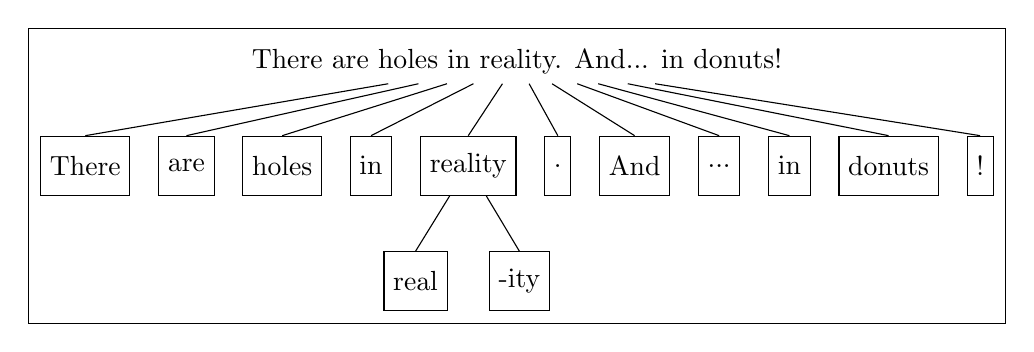
\begin{tikzpicture}[framed, x=1pt, y=1pt, yscale=-1, xscale=1, node distance=10pt]

    \node (start) at (0, 0) {};

    \node [draw, rectangle, align=center, minimum height=0.75cm, below left=20pt of start] (there) {There};
    % create another node on the right side with 10pt margin
    \node [draw, rectangle, align=center, minimum height=0.75cm, right=10pt of there] (are) {are};
    \node [draw, rectangle, align=center, minimum height=0.75cm, right=10pt of are] (holes) {holes};
    \node [draw, rectangle, align=center, minimum height=0.75cm, right=10pt of holes] (in) {in};
    \node [draw, rectangle, align=center, minimum height=0.75cm, right=10pt of in] (reality) {reality};
    \node [draw, rectangle, align=center, minimum height=0.75cm, right=10pt of reality] (dot) {.};
    \node [draw, rectangle, align=center, minimum height=0.75cm, right=10pt of dot] (and) {And};
    \node [draw, rectangle, align=center, minimum height=0.75cm, right=10pt of and] (dots) {...};
    \node [draw, rectangle, align=center, minimum height=0.75cm, right=10pt of dots] (in2) {in};
    \node [draw, rectangle, align=center, minimum height=0.75cm, right=10pt of in2] (donuts) {donuts};
    \node [draw, rectangle, align=center, minimum height=0.75cm, right=10pt of donuts] (exc) {!};

    \node [draw, rectangle, align=center, minimum height=0.75cm, below left=20pt and -10pt of reality] (real) {real};
    \node [draw, rectangle, align=center, minimum height=0.75cm, below right=20pt and -10pt of reality] (ity) {-ity};

    \node [align=center, anchor=center, anchor=south] (sentence) at ([yshift=-40pt]current bounding box.center) {There are holes in reality. And... in donuts!};

    \draw (sentence) -- (there.north);
    \draw (sentence) -- (are.north);
    \draw (sentence) -- (holes.north);
    \draw (sentence) -- (in.north);
    \draw (sentence) -- (reality.north);
    \draw (sentence) -- (dot.north);
    \draw (sentence) -- (and.north);
    \draw (sentence) -- (dots.north);
    \draw (sentence) -- (in2.north);
    \draw (sentence) -- (donuts.north);
    \draw (sentence) -- (exc.north);

    \draw (reality) -- (real.north);
    \draw (reality) -- (ity.north);
\end{tikzpicture}

\end{figure}

\subsection{$N$-gramas e Modelos de Predição de Palavras}

Os $N$-gramas, em NLP, são estruturas de agrupamento de palavras ou \textit{tokens} que desempenham um papel crucial na tarefa de previsão em textos. Tratam-se de uma junção de todos os elementos subjacentes possíveis, formando conjuntos de $n$ unidades. Essas representações são utilizadas, aliadas aos conceitos da teoria de Markov e das probabilidades, para treinar modelos simples de predição de palavras.

\begin{figure}[H]
    \centering
    \caption{Exemplos de $n$-gramas para $n=1, 2, 3$. Imagem extraída de \cite{fasttext-2018}.}
    \label{fig:bigrama}
    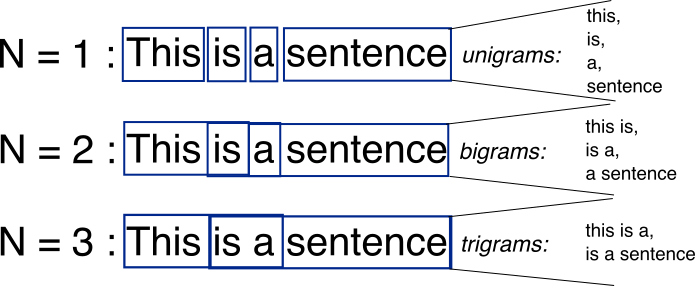
\includegraphics[width=0.6\textwidth]{../figuras/ngrams.png}
\end{figure}

O objetivo, nesse caso, é estimar a função de probabilidade $P(W_t | W_{t-(n-1)}, \cdots, W_{t-1})$, onde $W_t$ é a palavra atual e $W_{t-(n-1)}, \cdots, W_{t-1}$ representa o histórico de palavras. Sob a perspectiva estocástica, a classificação da história anterior ($W_{t-(n-1)}, \cdots, W_{t-1}$) é essencial para predizer as novas ocorrências, já que, com uma quantia suficientemente grande de textos, é possível estimar quais palavras tendem a aparecer em sequência.

No entanto, lidar com cada história textual separadamente é impraticável, já que é possível receber como entrada textos totalmente novos, sem construções de referência. A teoria de Markov, assim, surge como uma solução plausível, considerando que apenas o contexto local anterior, representado pelo conjunto das últimas palavras ($W_{t-(n-1)}, ..., W_{t-1}$), influencia a escolha da próxima ocorrência. Essa suposição leva em conta que a ordem de palavras em um texto é relevante e que geralmente existe maior correlação estatística entre unidades vizinhas, conforme pontuado em \cite{bengio-et-al-2003}.

Agrupando todas as histórias que compartilham as mesmas $n - 1$ palavras em uma mesma classe de equivalência, cria-se um modelo de Markov de ordem $n - 1$, conhecido como modelo de linguagem $N$-grama (\cite{manning-schuetze-1999}). Ao nomear tais modelos, a terminologia comumente utilizada refere-se a valores específicos de $n$, como bigrama para $n=2$ e trigrama para $n=3$. A abordagem de agrupar contextos semelhantes com base na teoria de Markov oferece uma maneira eficaz de prever palavras subsequentes em textos, com ampla aplicação no processamento de linguagem natural e análise de sentimentos.

\subsection{\textit{One-Hot Encodings}}

A técnica de \textit{one-hot encoding} é uma abordagem de representação palavras ou \textit{tokens} no âmbito do NLP. Nesse mecanismo, cada elemento do vocabulário é mapeado para um vetor binário distinto, onde todos os valores são zero, exceto aquele correspondente à posição da palavra de interesse, para a qual atribui-se o valor 1. Esse método cria representações vetoriais esparsas, cuja dimensionalidade é equivalente ao tamanho do vocabulário.

A principal característica do \textit{one-hot encoding} é a independência entre as representações de palavras. Cada uma delas é tratada como uma entidade única, sem consideração pela semelhança semântica ou relações contextuais com outras unidades do vocabulário. A representação binária resultante destaca a presença ou ausência de palavras específicas, mas não incorpora informações sobre o significado relativo delas ou suas interações semânticas.

Quando usado para codificar características ou classes, o \textit{one-hot encoding} pode ser considerado mais interpretável, dada sua natureza de independência explícita. A representação binária atribui um valor de 1 à categoria de interesse, com sua devida especificação, e 0 para todas as outras categorias, individualizando a presença ou ausência de uma característica e aumentando a interpretação de modelos, como mostrado por \citet{manai2023impact}.

Apesar de sua simplicidade e interpretabilidade, o \textit{one-hot encoding} apresenta desvantagens significativas em termos de eficiência computacional e capacidade de generalização. A representação esparsa resulta em um alto consumo de memória, especialmente em vocabulários extensos, e a falta de captura de relações semânticas limita sua utilidade em tarefas mais complexas de NLP.

\subsection{\textit{Word Embeddings}}

\textit{Word embeddings} referem-se a representações vetoriais de palavras que capturam relações semânticas e contextuais. Distintas dos $N$-gramas, que se restringem a contextos locais, essas representações incorporam informações abrangentes de todo o texto.

A origem dessas codificações remonta aos estágios iniciais dos modelos neurais probabilísticos de linguagem. Inspirados nas redes neurais de compressão de texto propostas por \citet{schmidhuber-heil-1996}, \citet{bengio-et-al-2003} conceberam um modelo de predição de palavras com uma estrutura análoga. Nesse trabalho, uma camada de projeção foi introduzida na rede neural, desempenhando o papel de mapear palavras para vetores de baixa dimensão.

Essa abordagem serviu como fundamento para o desenvolvimento de técnicas mais refinadas de \textit{word embedding}, que se disseminaram amplamente em aplicações de NLP. A representação matemática de palavras, expressa como vetores, proporciona não apenas manipulações computacionais eficientes, mas também a modelagem de aspectos semânticos pertinentes aos textos.

Lidar com representações vetoriais reais de palavras viabiliza a compreensão e exploração de relações semânticas complexas. Tais codificações permitem expressar analogias e operações sobre os elementos, como no exemplo da soma das palavras ``rei'' e ``mulher'', que resulta em vetores próximos da representação de ``rainha'' (\cite{mikolov-etal-2013-linguistic}).

\begin{figure}[ht]
    \centering
    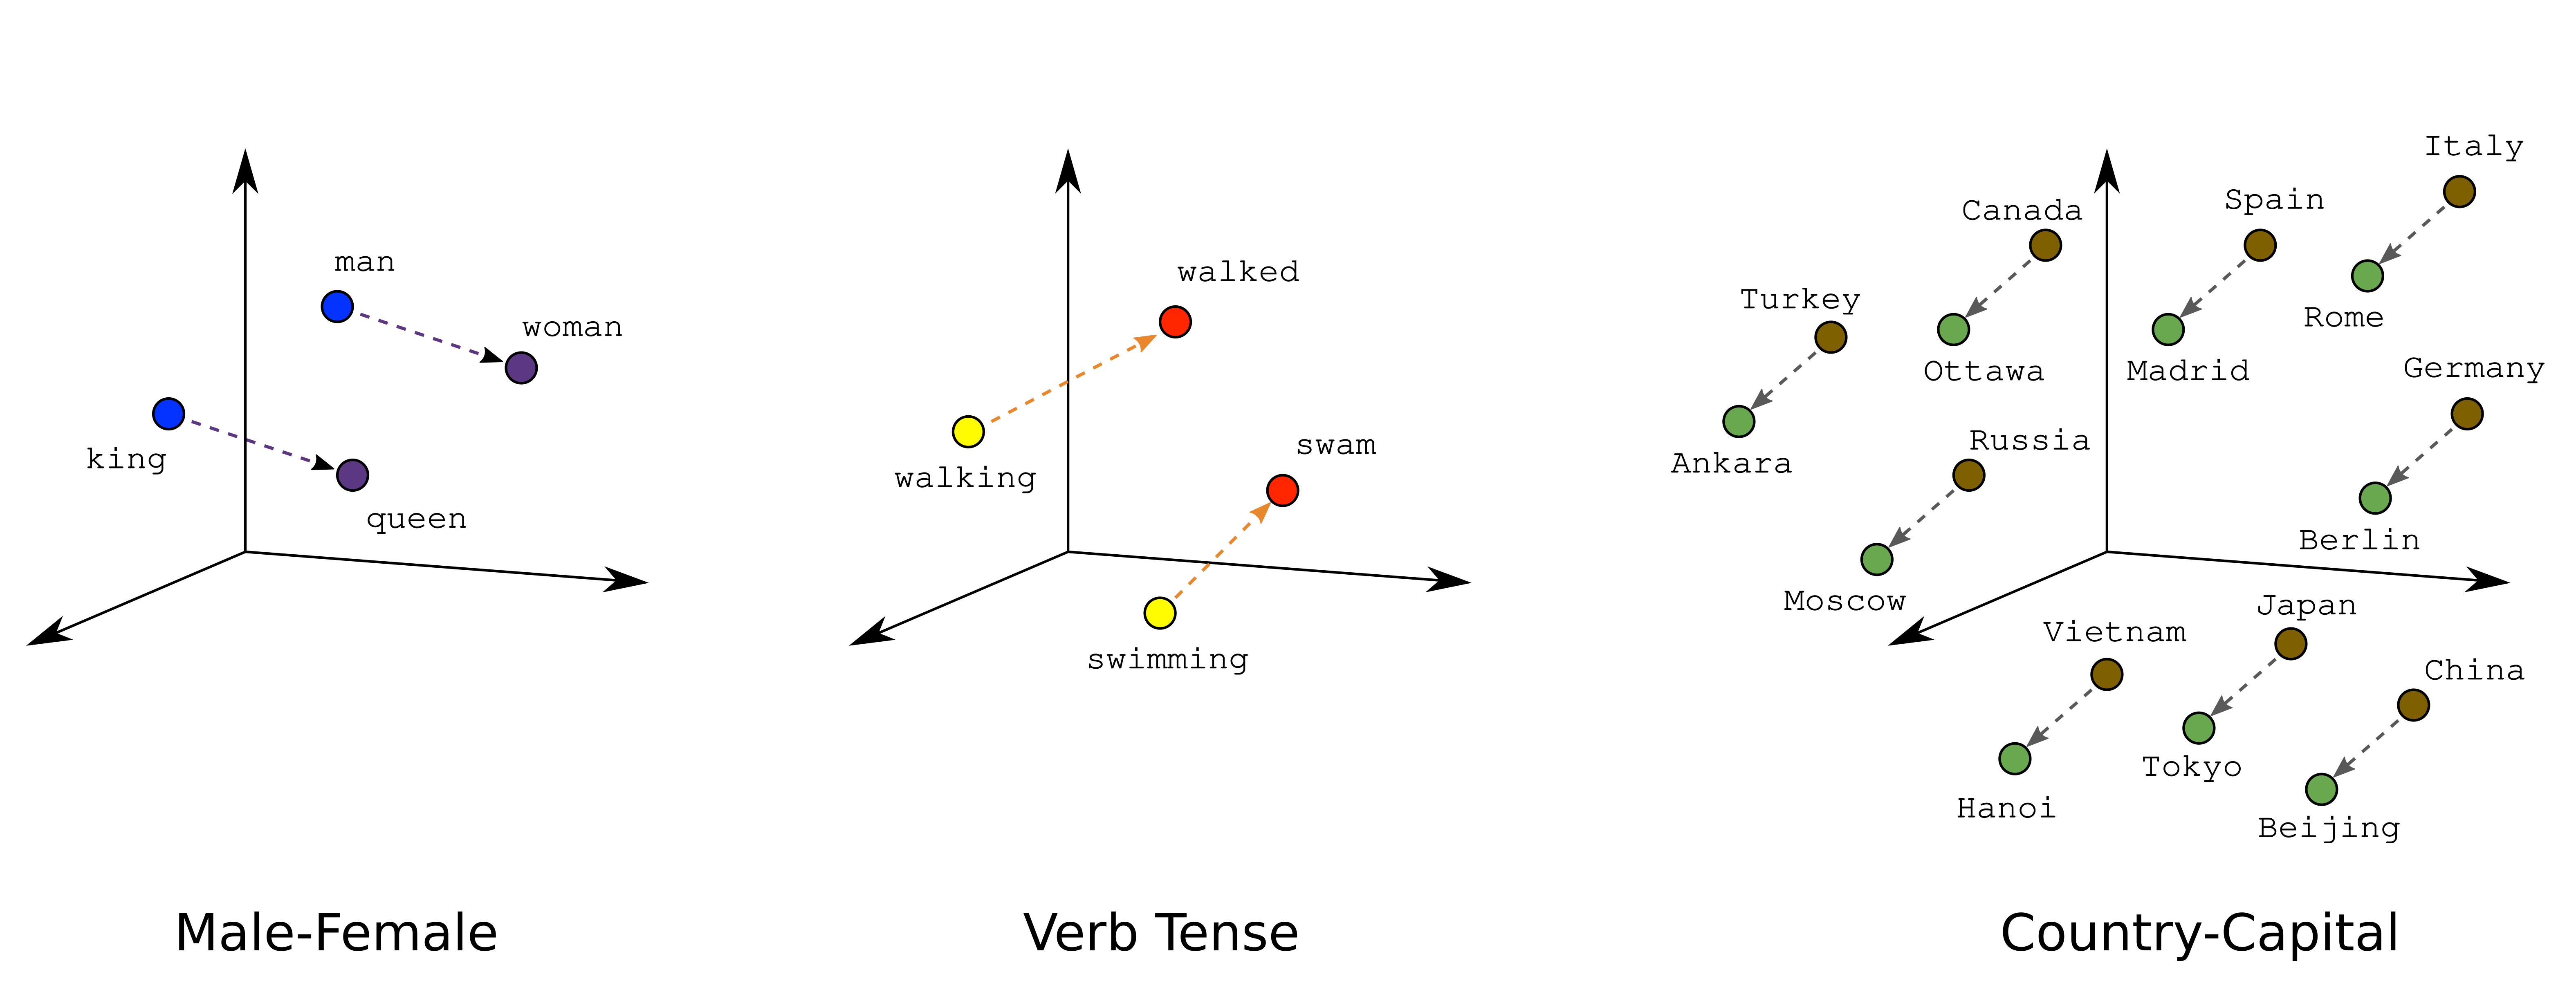
\includegraphics[width=\textwidth]{../figuras/wordembeddings.png}
    \caption{Representação vetorial de palavras sob alguns eixos semânticos. Imagem extraída de \url{https://developers.google.com/machine-learning/crash-course/embeddings/translating-to-a-lower-dimensional-space}}
    \label{fig:word_embeddings}
\end{figure}

O emprego de \textit{word embeddings} é, atualmente, mais frequente, já que o método confere vantagens significativas em termos de manipulação e compreensão semântica. Representações semelhantes a essa estrutura são empregadas em modelos de linguagem mais avançados, como o BERT. Três métodos notáveis de \textit{word embedding} são o Word2Vec, GloVe e FastText.

\subsubsection{Word2Vec}

O Word2Vec é uma técnica de \textit{word embedding} que realiza uma tradução de palavras para vetores em espaços contínuos. Este método, fundamentado em redes neurais, destaca-se por sua habilidade em preservar relações semânticas através de representações distribuídas (\cite{mikolov-etal-2013-linguistic}). O cerne do processo consiste na aprendizagem de representações que não apenas mapeiam palavras individuais, mas também capturam a proximidade semântica entre elas.

Essa codificação opera de modo a otimizar a representação vetorial de palavras com base em seu contexto geral, possibilitando a criação de \textit{embeddings} que capturam a semelhança lexical e aspectos relacionados ao significado. O modelo se destaca principalmente na incorporação de analogias e de consequências lógicas, tais quais ``\textbf{falar} está para \textbf{falado} como \textbf{escrever} está para \textbf{escrito}''.

\subsubsection{GloVe}

O GloVe (\textit{Global Vectors for Word Representation}) apresenta uma perspectiva distinta no panorama dos \textit{word embeddings}. Ele se destaca na geração de representações vetoriais fundamentadas em estatísticas globais de coocorrência de palavras em um \textit{corpus}. Essa abordagem permite uma visão abrangente das relações semânticas que transcendem contextos imediatos.

A metodologia do GloVe se baseia na construção de uma matriz de coocorrência, refletindo a probabilidade de duas palavras aparecerem juntas em um dado contexto (\cite{pennington-etal-2014-glove}). Por meio de técnicas algébricas, o modelo é usado para derivar \textit{embeddings} que melhor representem as relações semânticas capturadas por essa matriz. Dessa forma, transcende-se a limitação de representar palavras isoladamente, proporcionando uma visão holística das conexões semânticas de um texto.

\subsubsection{FastText}

O FastText, uma extensão evolutiva do Word2Vec, é um tipo de codificação que atua em nível de subpalavras. Cada palavra, nesse método, é representada por $n$-gramas de suas composições. Essa inovação confere à técnica uma notável flexibilidade na manipulação de palavras desconhecidas, capturando informações semânticas em camadas mais inferiores de um texto, e permite uma maior agilidade no processo de treinamento.

Considerar subpalavras no processo de geração de \textit{embeddings} capacita o FastText a representar os vocábulos como combinações de suas partes constituintes. Para a palavra \textit{where}, por exemplo, esse modelo pode considerar os trigramas \texttt{<wh, whe, her, ere, re>}, conforme delineado por \citet{bojanowski-etal-2016-enriching}. Isso se revela particularmente valioso em línguas com estrutura morfológica complexa, como a língua portuguesa, onde as palavras são formadas por múltiplos elementos significativos. Alguns vocábulos não conhecidos, nesse caso, podem ser construídos pelos $n$-gramas, dando poder de generalização ao modelo.

Além disso, o FastText possui uma eficácia singular no processo de treinamento, permitindo a criação de \textit{embeddings} em ambientes computacionais mais simples. Conforme evidenciado por \citet{joulin-etal-2016-bag}, métodos baseados em convoluções, tais quais os utilizados para treinar representações de Word2Vec, demonstram ser muito mais lentos que o FastText, que alcança tempos de treinamento da ordem de minutos em CPUs padrões de 20 \textit{threads}. Essa notável agilidade contribui significativamente para a adoção do FastText em tarefas de NLP que exijam rápidas codificações.

\section{Modelos de Linguagem Neurais}

Os modelos de linguagem neurais são uma classe de entidades estatísticas que atribuem probabilidades a cadeias de palavras. Em geral, dado uma sequência de $t$ \textit{tokens} $\boldsymbol{W} = w_{1}, \cdots, w_{t}$ e um vocabulário de tamanho $V$, atuam de modo a aproximar a função de distribuição de probabilidades de um novo \textit{token} $w_{t+1}$, indicado por $P(w_{t+1} | W)$ (\cite{sun-iyyer-2021}). Esses modelos utilizam uma função de composição, denotada por $h$, que é aplicada sobre a sequência $W$, produzindo uma saída $\boldsymbol{s} = h(\boldsymbol{W})$.

Como o intuito é obter uma aproximação da distribuição de probabilidades sobre o vocabulário, uma restrição fundamental é a de que a resposta $\boldsymbol{r}$ atribuída pelos modelos de linguagem, com $\boldsymbol{r} = (r_{1}, \cdots, r_{V}) \in \mathbb{R}^{V}$, tenha valores cuja soma total seja igual a 1. Para tal, utiliza-se, comumente, a função \textit{softmax} (\cite{softmax-bridle}), cujo objetivo é normalizar um vetor $\boldsymbol{z} = (z_{1}, \cdots, z_{n}) \in \mathbb{R}^{n}$:

\begin{equation}
    \label{eq:softmax}
    g(z_i) = \frac{e^{z_i}}{\sum_{j=1}^{n} e^{z_j}} \text{ , para todo $i \in \{1, \cdots, n\}$}
\end{equation}

A saída $\boldsymbol{s}$ é, então, utilizada para estimar a probabilidade de ocorrência de um novo \textit{token} $w_{t+1}$, conforme a equação \ref{eq:softmax}, a partir do mapeamento realizado por $g$. Esse processo gera a resposta $r = \widehat{P}(w_{t+1} | W)$, um vetor de distribuição de probabilidades aproximada para o \textit{token} $w_{t+1}$ sobre o vocabulário.

\subsection{Redes Neurais Tradicionais}

As redes neurais tradicionais foram as pioneiras no desenvolvimento de modelos de linguagem. Os autores \citet{bengio-et-al-2003} foram os primeiros a lidar com essa estrutura, propondo uma arquitetura mais simples com duas camadas principais. A primeira delas realiza uma tarefa de projeção, mapeando palavras para vetores de baixa dimensão. Já a segunda atua como uma camada oculta, que recebe uma sequência de vetores e produz uma saída com base em uma função de ativação.

A rede recebe como entrada representações em \textit{one-hot encoding} de palavras, que são multiplicadas por uma matriz de projeção $C \in \mathbb{R}^{d \times V}$, onde $d$ é a dimensão dos vetores de projeção e $V$ é o tamanho do vocabulário. Essa matriz é treinada para realizar o mapeamento linear de palavras para vetores de representação distribuída, como os \textit{word embeddings}. A saída da camada de projeção é uma matriz $X \in \mathbb{R}^{d \times t}$, onde $t$ é o tamanho da sequência de entrada.

A matriz $X$ é, então, utilizada como entrada para a camada oculta, composta por uma quantia fixa de unidades de processamento, convencionalmente chamadas de neurônios. Cada neurônio recebe a sequência de vetores $x_{i} \in \mathbb{R}^{d}$ e produz uma saída $h_{i} \in \mathbb{R}^{d}$, calculada por:

\begin{equation}
    \label{eq:nnlm}
    h_{i}(x_{i}) = \tanh \left( b + W x_{i} \right)
\end{equation}

onde $W \in \mathbb{R}^{d \times d}$ é uma matriz de pesos e $b \in \mathbb{R}^{d}$ é um vetor de viés. A saída dessa etapa, representada pela matriz $H \in \mathbb{R}^{d \times t}$, passa por uma camada de tratamento com a função \textit{softmax} (\ref{eq:softmax}), gerando, finalmente, um vetor que representa a aproximação da função de probabilidades.

A Figura \ref{fig:nnlm} ilustra a estrutura dessa rede neural:

\begin{figure}[H]
    \centering
    \caption{Arquitetura de uma rede neural tradicional para modelagem de linguagem. Imagem extraída de \cite{bengio-et-al-2003}.}
    \label{fig:nnlm}
    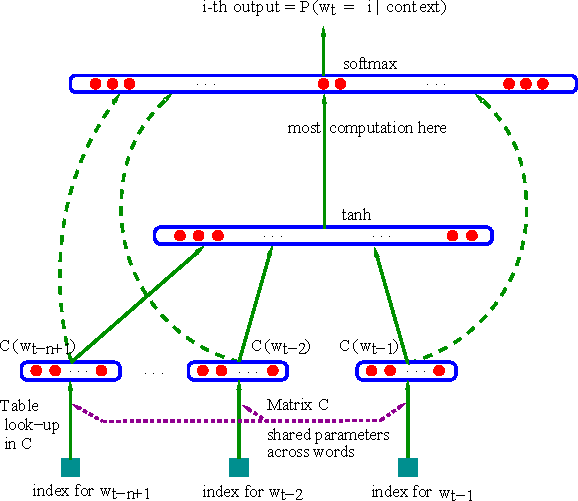
\includegraphics[width=0.6\textwidth]{../figuras/nnlm.pdf}
\end{figure}

O treinamento dessa arquitetura de redes neurais tradicionais, apresentada por \citet{bengio-et-al-2003}, é realizado por meio da busca iterativa do valor $\theta$ que maximize a verossimilhança em relação às probabilidades logarítmiticas de um \textit{corpus} de tamanho $T$, representada pela equação \ref{eq:loglikelihood}. O algoritmo utilizado para essa busca é o de subida estocástica do gradiente (\cite{machine-learning-in-action}).

\begin{equation}
    \label{eq:loglikelihood}
    \mathcal{L}(\theta) = \frac{1}{T}\sum_{t=1}^{T} \log \widehat{P}(w_{t} | w_{t-1}, \cdots, w_{1}; \theta)
\end{equation}

À época, esses modelos representaram um marco importante no âmbito do NLP. Além da abordagem pioneira na representação de palavras, futuramente estabelecidos como os \textit{embeddings}, sua capacidade de aprender funções que estimam probabilidades oferece uma base sólida para a compreensão e geração de linguagem.

Todavia, a utilização dessa abordagem para lidar com textos suscitou muitas limitações na área. Uma delas é a incapacidade de capturar a dependência temporal entre as palavras em uma sequência, já que essas redes processam cada entrada de forma independente, sem considerar a ordem ou a relação cronológica entre vocábulos. Isso dificulta o uso do modelo para análise de textos cuja estrutura sequencial é essencial para o entendimento, como na avaliação automática de redações.

Outro desafio enfrentado pelas redes neurais tradicionais é a dificuldade em lidar com \textit{corpus} de diferentes comprimentos. Como essas estruturas têm uma arquitetura fixa com um número predefinido de camadas e unidades, torna-se custoso processar sequências de diferentes tamanhos de forma eficiente, já que o modelo possui uma complexidade computacional exponencial em relação ao tamanho da entrada.

\subsection{Redes Neurais Recorrentes (RNN)}

Para superar as limitações das redes neurais tradicionais em representar relações temporais e de ordem, surgiram as Redes Neurais Recorrentes (RNNs), baseadas na arquitetura proposta por \citet{rumelhart-1986-learning}. As RNNs têm a habilidade de aprender padrões de qualquer sequência de dados, como genomas, séries temporais, entre outros. Tal capacidade as torna particularmente adequadas para lidar, também, com tarefas de compreensão de textos, tendo em vista o caráter sequencial dessas estruturas (\cite{zhang2023dive}).

A arquitetura se diferencia principalmente pela introdução de um componente de memória, que é atualizado a cada novo elemento da sequência. A cada passo, a saída gerada pela rede realimenta a entrada, fazendo com que as RNNs levem em conta não só o novo dado, mas também as informações já processadas anteriormente. Assim, para um passo de tempo $t$ e uma função de ativação $f$, a saída da rede $h_t$ é calculada pela equação \ref{eq:rnn}:

\begin{equation}
    \label{eq:rnn}
    h_t = f(\boldsymbol{W}_{ih} x_t + \boldsymbol{b}_{ih} + \boldsymbol{W}_{hh} h_{t-1} + \boldsymbol{b}_{hh})
\end{equation}

em que $x_t$ é a entrada no tempo $t$, $\boldsymbol{W}_{ih}$ os pesos da camada oculta, $\boldsymbol{W}_{hh}$ os pesos da ciclagem de informação (de camada oculta para camada oculta), $\boldsymbol{b}_{ih}$ os vieses referentes à entrada atual e $\boldsymbol{b}_{hh}$ os vieses relacionados com o histórico temporal. O termo $h_{t-1}$ representa o estado oculto anterior, incorporando informações das etapas de tempo passadas.

\begin{figure}[H]
    \centering
    \caption{Arquitetura de uma RNN em formato simplificado e em formato sequencial aberto. Imagem adaptada de \cite{zhang2023dive}.}
    \label{fig:rnns}
    \usetikzlibrary{positioning,chains}
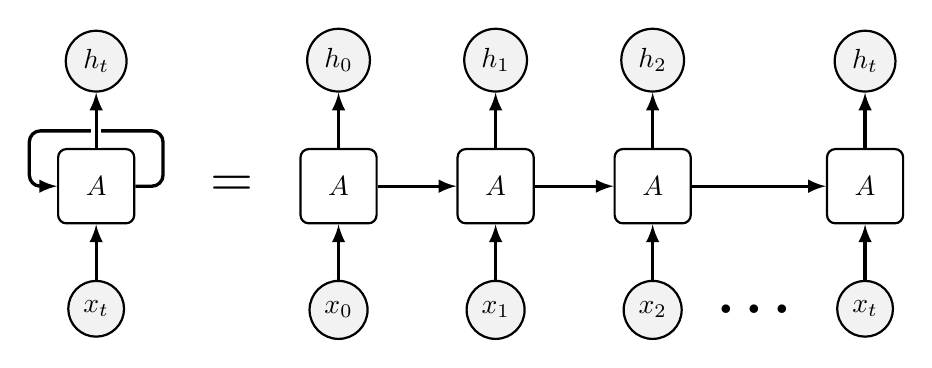
\begin{tikzpicture}[item/.style={circle,draw,thick,align=center},
itemc/.style={draw,thick,align=center,inner sep=1em,rounded corners=0.3em},
itema/.style={itemc,on chain,join},]
 \begin{scope}[start chain=going right,nodes=itema,every
 join/.style={-latex,very thick},local bounding box=chain]
 \path node (A0) {$A$} node (A1) {$A$} node (A2) {$A$} node[xshift=2em] (At)
 {$A$};
 \end{scope}
 \node[left=1em of chain,scale=2] (eq) {$=$};
 \node[left=2em of eq,itemc] (AL) {$A$};
 \path (AL.west) ++ (-1em,2em) coordinate (aux);
 \draw[very thick,-latex,rounded corners] (AL.east) -| ++ (1em,2em) -- (aux)
 |- (AL.west);
 \foreach \X in {0,1,2,t}
 {\draw[very thick,-latex] (A\X.north) -- ++ (0,2em)
 node[above,item,fill=gray!10] (h\X) {$h_\X$};
 \draw[very thick,latex-] (A\X.south) -- ++ (0,-2em)
 node[below,item,fill=gray!10] (x\X) {$x_\X$};}
 \draw[white,line width=0.8ex] (AL.north) -- ++ (0,1.9em);
 \draw[very thick,-latex] (AL.north) -- ++ (0,2em)
 node[above,item,fill=gray!10] {$h_t$};
 \draw[very thick,latex-] (AL.south) -- ++ (0,-2em)
 node[below,item,fill=gray!10] {$x_t$};
 \path (x2) -- (xt) node[midway,scale=2,font=\bfseries] {\dots};
\end{tikzpicture}

\end{figure}

Para o treinamento, as RNNs utilizam o algoritmo \textit{backpropagation through time} (BPTT), que é uma variação do algoritmo de retropropagação de redes tradicionais (\cite{schmidt2019recurrent}). O BPTT, de modo geral, atua criando uma versão sequencial aberta das RNNs ao longo do tempo, conforme mostrado na figura \ref{fig:rnns}. Essa representação é, então, tratada como uma estrutura tradicional, permitindo a aplicação do algoritmo de \textit{backpropagation} comum.

Algumas variações de RNNs, como as \textit{Bidirectional Recurrent Neural Networks} (BRNN), também surgiram para atender outras demandas específicas da área de NLP, como a previsão de palavras em meio de sequências. Esses modelos incorporam a capacidade de processar a informação tanto no sentido direto quanto no inverso, permitindo que a previsão de uma palavra considere não apenas o contexto precedente, mas também o subsequente. A estrutura esquemática das BRNNs pode ser vista na figura \ref{fig:brnn}.

\begin{figure}[H]
    \centering
    \caption{Arquitetura de uma \textit{Bidirectional Recurrent Neural Network} (BRNN). Imagem adaptada de \cite{zhang2023dive}.}
    \label{fig:brnn}
    % Adapted from PetarV-/TikZ repository @ GitHub
\usetikzlibrary{positioning}

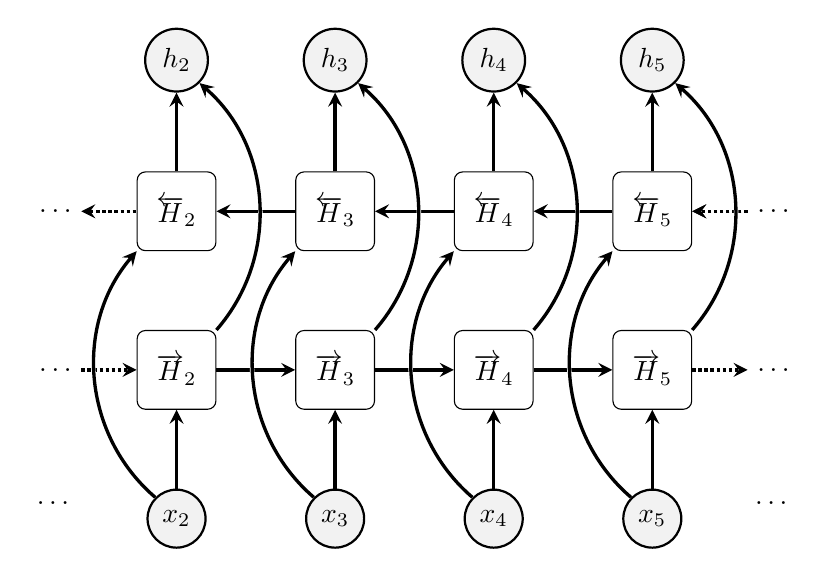
\begin{tikzpicture}[
        inout/.style={circle, draw, fill=gray!10, thick, align=center},
        hid/.style={inner sep=0.2em,rounded corners=0.3em},
    ]
	\node[rectangle] (Y0) at (0, 0) {$\dots$};
    \node[hid, rectangle, draw, right=2em of Y0, minimum height=1cm, minimum width=1cm] (RNN) {$\overrightarrow{H}_{2}$};
    \node[hid, rectangle, right=of RNN, draw, minimum height=1cm, minimum width=1cm] (RNN2) {$\overrightarrow{H}_{3}$};
    \node[hid, rectangle, right=of RNN2, draw, minimum height=1cm, minimum width=1cm] (RNN3) {$\overrightarrow{H}_{4}$};

    \node[hid, rectangle, right= of RNN3, draw, minimum height=1cm, minimum width=1cm] (RNN4) {$\overrightarrow{H}_{5}$};
	\node[rectangle, right=2em of RNN4] (RNN5) {$\dots$};


    \node[hid, rectangle, above=of RNN4, draw, minimum height=1cm, minimum width=1cm] (R25) {$\overleftarrow{H}_{5}$};
    \node[hid, rectangle, left=of R25, minimum height=1cm, minimum width=1cm, draw] (R24) {$\overleftarrow{H}_{4}$};
    \node[hid, rectangle, left=of R24, draw, minimum height=1cm, minimum width=1cm] (R23) {$\overleftarrow{H}_{3}$};
    \node[hid, rectangle, left=of R23, draw, minimum height=1cm, minimum width=1cm] (R22) {$\overleftarrow{H}_{2}$};
    \node[rectangle, left=2em of R22] (R21) {$\dots$};
	\node[right=2em of R25] (Y20) {$\dots$};

	\node[inout, below=of RNN] (X1) {$x_2$};
	\node[inout, below=of RNN2] (X2) {$x_3$};
	\node[inout, below=of RNN3] (X3) {$x_4$};
	\node[inout, below=of RNN4] (X4) {$x_5$};
	\node[inout, above=of R25] (Y5) {$h_5$};
	\node[inout, above=of R24] (Y4) {$h_4$};
	\node[inout, above=of R23] (Y3) {$h_3$};
	\node[inout, above=of R22] (Y2) {$h_2$};

	\draw[-stealth, very thick] (X1) -- (RNN);
	\draw[-stealth, very thick] (X2) -- (RNN2);
	\draw[-stealth, very thick] (X3) -- (RNN3);
	\draw[-stealth, very thick] (X4) -- (RNN4);
	\draw[-stealth, very thick, densely dotted] (Y0) -- (RNN);
	\draw[-stealth, very thick] (RNN) -- (RNN2);
	\draw[-stealth, very thick] (RNN2) -- (RNN3);
	\draw[-stealth, very thick] (RNN3) -- (RNN4);
	\draw[-stealth, densely dotted, very thick] (RNN4) -- (RNN5);
	\node[below=4em of Y0] (d) {\dots};
	\node[below=4em of RNN5] (d) {\dots};

	\path[-stealth, ultra thick, white] (X1) edge[bend left=45] (R22);
	\path[-stealth, very thick] (X1) edge[bend left=45] (R22);
	\path[-stealth, ultra thick, white] (X2) edge[bend left=45] (R23);
	\path[-stealth, very thick] (X2) edge[bend left=45] (R23);
	\path[-stealth, ultra thick, white] (X3) edge[bend left=45] (R24);
	\path[-stealth, very thick] (X3) edge[bend left=45] (R24);
	\path[-stealth, ultra thick, white] (X4) edge[bend left=45] (R25);
	\path[-stealth, very thick] (X4) edge[bend left=45] (R25);
	\draw[-stealth, densely dotted, very thick] (Y20) -- (R25);

	\draw[-stealth, very thick] (R22) -- (Y2);
	\draw[-stealth, very thick] (R23) -- (Y3);
	\draw[-stealth, very thick] (R24) -- (Y4);
	\draw[-stealth, very thick] (R25) -- (Y5);

	\draw[stealth-, densely dotted, very thick] (R21) -- (R22);
	\draw[stealth-, very thick] (R22) -- (R23);
	\draw[stealth-, very thick] (R23) -- (R24);
	\draw[stealth-, very thick] (R24) -- (R25);
	\draw[-stealth, densely dotted, very thick] (Y20) -- (R25);

	\path[-stealth, ultra thick, white] (RNN) edge[bend right=45] (Y2);
	\path[-stealth, very thick] (RNN) edge[bend right=45] (Y2);
	\path[-stealth, ultra thick, white] (RNN2) edge[bend right=45] (Y3);
	\path[-stealth, very thick] (RNN2) edge[bend right=45] (Y3);
	\path[-stealth, ultra thick, white] (RNN3) edge[bend right=45] (Y4);
	\path[-stealth, very thick] (RNN3) edge[bend right=45] (Y4);
	\path[-stealth, ultra thick, white] (RNN4) edge[bend right=45] (Y5);
	\path[-stealth, very thick] (RNN4) edge[bend right=45] (Y5);
\end{tikzpicture}

\end{figure}

A possibilidade de manter estados internos ao longo das sequências permite que as RNNs capturem dependências de longo alcance em textos, um desafio enfrentado pelas redes neurais tradicionais. Além disso, a abordagem temporal habilita a utilização delas em \textit{corpus} de tamanhos variáveis, garantindo que se adaptem a diferentes contextos.

No entanto, a arquitetura recorrente também apresenta desafios, sendo o mais proeminente o problema de desvanecimento ou explosão do gradiente. Durante o treinamento, os vetores responsáveis por minimizar a função de perda podem se tornar extremamente pequenos ou grandes, dificultando a atualização eficiente dos parâmetros da rede. Por estarem associadas aos pesos da camada oculta, essas variações resultam em dificuldades para aprender dependências temporais de longo prazo, já que o histórico pode ser pouco relevante ou muito influente, a depender dos gradientes. Isso compromete principalmente a capacidade da RNN de reter informações pertinentes em sequências extensas, como já pontuado por \citet{schmidt2019recurrent}.

Ademais, as redes neurais recorrentes podem ser consideradas ineficientes e pouco escaláveis em relação a outras abordagens. Devido ao seu caráter sequencial, elas não conseguem processar entradas paralelamente, o que aumenta o tempo de treino de forma substancial.

Para superar o problema do desvanecimento do gradiente, foram propostas variantes de RNNs, como as redes \textit{Long Short-Term Memory} (LSTM) e as \textit{Gated Recurrent Units} (GRU).

\subsubsection{\textit{Long Short-Term Memory} (LSTM)}

As LSTMs são arquiteturas de RNNs que introduzem unidades de memória atualizadas e controladas por meio de portas (\cite{hochreiter1997long}). Isso permite que elas capturem relações de longo prazo em sequências sem uma propagação de erros que cresça descomedidamente, tornando-as especialmente eficazes em tarefas de NLP que usam a abordagem recorrente.

A estrutura de uma LSTM é formada por células de memória, que são envolvidas por três portas: de entrada ($\boldsymbol{I}_{t}$), esquecimento ($\boldsymbol{F}_{t}$) e saída ($\boldsymbol{O}_{t}$). A porta de entrada controla a atualização da célula de memória, a de esquecimento regula a retenção de informações em relação às computações anteriores e a de saída determina o valor final da unidade.

\begin{equation}
    \label{eq:lstm_input}
    \boldsymbol{I}_{t} = f \left( \boldsymbol{W}_{xi} \boldsymbol{X}_{t} + \boldsymbol{W}_{hi} \boldsymbol{H}_{t-1} + \boldsymbol{b}_{i} \right)
\end{equation}
\begin{equation}
    \label{eq:lstm_forget}
    \boldsymbol{F}_{t} = f \left( \boldsymbol{W}_{xf} \boldsymbol{X}_{t} + \boldsymbol{W}_{hf} \boldsymbol{H}_{t-1} + \boldsymbol{b}_{f} \right)
\end{equation}
\begin{equation}
    \label{eq:lstm_output}
    \boldsymbol{O}_{t} = f \left( \boldsymbol{W}_{xo} \boldsymbol{X}_{t} + \boldsymbol{W}_{ho} \boldsymbol{H}_{t-1} + \boldsymbol{b}_{o} \right)
\end{equation}

As portas são calculadas pelas equações \ref{eq:lstm_input}, \ref{eq:lstm_forget} e \ref{eq:lstm_output}, respectivamente, em que $\boldsymbol{W}_{xi}$, $\boldsymbol{W}_{hi}$, $\boldsymbol{W}_{xf}$, $\boldsymbol{W}_{hf}$, $\boldsymbol{W}_{xo}$ e $\boldsymbol{W}_{ho}$ são matrizes de pesos e $\boldsymbol{b}_{i}$, $\boldsymbol{b}_{f}$ e $\boldsymbol{b}_{o}$ são vetores de viés. A função de ativação $f$ utilizada nas portas é a sigmoide, dada pela equação \ref{eq:sigmoid}, que retorna valores entre 0 e 1. Ela é utilizada para controlar a quantidade de informação que deve ser passada para a célula de memória.

\begin{equation}
    \label{eq:sigmoid}
    f(x) = \frac{1}{1 + e^{-x}}
\end{equation}

Conforme pontuado em \cite{schmidt2019recurrent}, as LSTMs têm, ainda, um componente de memória $\boldsymbol{\tilde{C}}_{t}$, cuja atualização é controlada pela combinação com as portas da célula. O principal objetivo desse elemento é regular a quantia de informação que deve ser passada para um novo estado de memória $\boldsymbol{C}_{t}$ com base no estado anterior $\boldsymbol{C}_{t-1}$. O cálculo de $\boldsymbol{\tilde{C}}_{t}$ é dado pela equação \ref{eq:lstm_ctilde}:

\begin{equation}
    \label{eq:lstm_ctilde}
    \boldsymbol{\tilde{C}}_{t} = \tanh \left( \boldsymbol{W}_{xc} \boldsymbol{X}_{t} + \boldsymbol{W}_{hc} \boldsymbol{H}_{t-1} + \boldsymbol{b}_{c} \right)
\end{equation}

em que $\boldsymbol{W}_{xc}$ e $\boldsymbol{W}_{hc}$ são matrizes de pesos e $\boldsymbol{b}_{c}$ é um vetor de viés. A função de ativação de tangente hiperbólica é utilizada para normalizar os valores da célula de memória, retornando valores entre -1 e 1. Por fim, o estado interno da célula de memória $\boldsymbol{C}_{t}$ é calculado pela expressão \ref{eq:lstm_c} e a saída da unidade $\boldsymbol{H}_{t}$ é dada pela equação \ref{eq:lstm_h}, em que $\odot$ é a multiplicação elemento a elemento, chamada de produto de Hadamard.

\begin{equation}
    \label{eq:lstm_c}
    \boldsymbol{C}_{t} = \boldsymbol{F}_{t} \odot \boldsymbol{C}_{t-1} + \boldsymbol{I}_{t} \odot \boldsymbol{\tilde{C}}_{t}
\end{equation}

\begin{equation}
    \label{eq:lstm_h}
    \boldsymbol{H}_{t} = \boldsymbol{O}_{t} \odot \tanh(\boldsymbol{C}_{t})
\end{equation}

A Figura \ref{fig:lstm_architecture} ilustra a arquitetura geral das LSTMs.

\begin{figure}[H]
    \centering
    \caption{Arquitetura de uma célula de memória das redes \textit{Long Short-Term Memory} (LSTM) em um dado tempo. Imagem adaptada de \cite{zhang2023dive}.}
    \label{fig:lstm_architecture}
    % Adapted from J. Leon, https://tex.stackexchange.com/questions/432312/how-do-i-draw-an-lstm-cell-in-tikz
\usetikzlibrary{positioning, fit, arrows.meta, shapes}

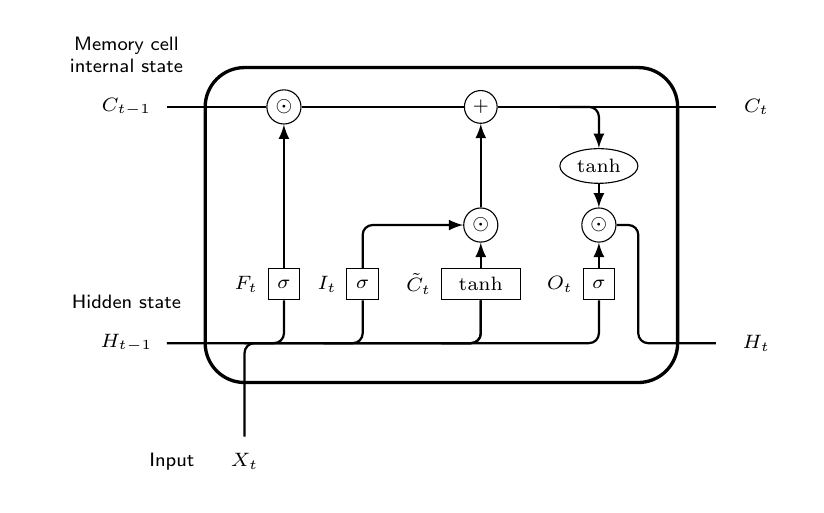
\begin{tikzpicture}[
    font=\sf \scriptsize,
    >=latex,
    % Styles
    cell/.style={
        rectangle,
        rounded corners=5mm,
        draw,
        very thick,
        },
    operator/.style={
        circle,
        draw,
        inner sep=1.5pt,
        minimum height =0.4cm,
        },
    function/.style={
        ellipse,
        draw,
        inner sep=2pt
        },
    ct/.style={
        line width = .75pt,
        minimum height=0.60cm,
        minimum width=1cm,
        inner sep=2pt,
        },
    gt/.style={
        rectangle,
        draw,
        minimum width=0.4cm,
        minimum height=0.4cm,
        inner sep=2pt
        },
    inoutlabels/.style={
        text width=2cm,
        align=center,
        },
    Arrow/.style={
        rounded corners=.125cm,
        thick,
        },
    ]

    \node [cell, minimum height =4cm, minimum width=6cm] at (0,0){} ;

    \node [gt, label={left:$\boldsymbol{F}_{t}$}] (ibox1) at (-2,-0.75) {$\sigma$};
    \node [gt, label={left:$\boldsymbol{I}_{t}$}] (ibox2) at (-1,-0.75) {$\sigma$};
    \node [gt, minimum width=1cm, label={left:$\boldsymbol{\tilde{C}}_{t}$}] (ibox3) at (0.5,-0.75) {$\tanh$};
    \node [gt, label={left:$\boldsymbol{O}_{t}$}] (ibox4) at (2,-0.75) {$\sigma$};

    \node [operator] (mux1) at (-2,1.5) {$\odot$};
    \node [operator] (add1) at (0.5,1.5) {+};
    \node [operator] (mux2) at (0.5,0) {$\odot$};
    \node [operator] (mux3) at (2,0) {$\odot$};
    \node [function] (func1) at (2,0.75) {$\tanh$};

    \node[ct, label={[inoutlabels]Memory cell internal state}] (c) at (-4,1.5) {$\boldsymbol{C}_{t-1}$};
    \node[ct, label={[inoutlabels]Hidden state}] (h) at (-4,-1.5) {$\boldsymbol{H}_{t-1}$};
    \node[ct, label={[inoutlabels, align=right]left:Input}] (x) at (-2.5,-3) {$\boldsymbol{X}_{t}$};

    \node[ct] (c2) at (4,1.5) {$\boldsymbol{C}_{t}$};
    \node[ct] (h2) at (4,-1.5) {$\boldsymbol{H}_{t}$};

    \draw [Arrow] (c) -- (mux1) -- (add1) -- (c2);

    \draw [Arrow] (h) -| (ibox4);
    \draw [Arrow] (h -| ibox1)++(-0.5,0) -| (ibox1);
    \draw [Arrow] (h -| ibox2)++(-0.5,0) -| (ibox2);
    \draw [Arrow] (h -| ibox3)++(-0.5,0) -| (ibox3);
    \draw [Arrow] (x) -- (x |- h)-| (ibox3);

    \draw [->, Arrow] (ibox1) -- (mux1);
    \draw [->, Arrow] (ibox2) |- (mux2);
    \draw [->, Arrow] (ibox3) -- (mux2);
    \draw [->, Arrow] (ibox4) -- (mux3);
    \draw [->, Arrow] (mux2) -- (add1);
    \draw [->, Arrow] (add1 -| func1)++(-0.5,0) -| (func1);
    \draw [->, Arrow] (func1) -- (mux3);

    \draw [-, Arrow] (mux3 |- h2)++(0.5,0.5) |- (h2);
    \draw [-, Arrow] (mux3 |- h2)++(0.5,0.5) |- (mux3);
\end{tikzpicture}

\end{figure}

A capacidade de aprender dependências de longo prazo em sequências destaca as LSTMs das redes neurais recorrentes convencionais. A estrutura de memória permite que elas capturem relações entre elementos distantes em uma sequência sem que o gradiente desvaneça ou cresça excessivamente. Isso é, em particular, importante para lidar com textos extensos, como os de uma redação.

Entretanto, as LSTMs não são isentas de desvantagens. Uma delas é a complexidade computacional, já que a estrutura de memória e as portas adicionam uma quantidade considerável de parâmetros ao modelo. Somado a isso, assim como no caso das RNNs convencionais, a arquitetura sequencial dessas redes não permite um processamento paralelo, agravando o problema de eficiência no treino.

\subsubsection{\textit{Gated Recurrent Unit} (GRU)}

Outra variação de RNNs é a \textit{Gated Recurrent Unit} (GRU), que visa simplificar a arquitetura das LSTMs, mantendo uma desempenho de avaliação semelhante. A GRU possui menos parâmetros e apenas duas portas: uma de atualização e uma de reinício (\cite{cho2014learning}). Isso a torna mais eficiente em termos computacionais e, em muitos casos, tão eficaz quanto as LSTMs.

A estrutura de uma GRU possui unidades de memória controladas por duas portas principais: a de atualização $\boldsymbol{Z}_{t}$ e a de reinício $\boldsymbol{R}_{t}$. Elas regulam o fluxo de informação de maneira eficiente à medida que atuam com menos parâmetros, sem perder a propriedade das LSTMs de assimilação de relações a longo prazo.

Em geral, a porta de atualização ajuda a capturar as dependências de longo prazo, enquanto a de reinício auxilia na modelagem das dependências de curto prazo. A primeira é calculada pela equação \ref{eq:gru_update} e a segunda pela equação \ref{eq:gru_reset}:

\begin{equation}
    \label{eq:gru_update}
    \boldsymbol{Z}_{t} = f \left( \boldsymbol{W}_{xr} \boldsymbol{X}_{t} + \boldsymbol{W}_{hr} \boldsymbol{H}_{t-1} + \boldsymbol{b}_{r} \right)
\end{equation}
\begin{equation}
    \label{eq:gru_reset}
    \boldsymbol{R}_{t} = f \left( \boldsymbol{W}_{xz} \boldsymbol{X}_{t} + \boldsymbol{W}_{hz} \boldsymbol{H}_{t-1} + \boldsymbol{b}_{z} \right)
\end{equation}

em que $\boldsymbol{W}_{xr}$, $\boldsymbol{W}_{hr}$, $\boldsymbol{W}_{xz}$ e $\boldsymbol{W}_{hz}$ são matrizes de pesos, $\boldsymbol{b}_{r}$ e $\boldsymbol{b}_{z}$ são vetores de viés e $f$ é a função de ativação sigmoide (\ref{eq:sigmoid}). Ambas as expressões são utilizadas para calcular um estado oculto intermediário $\tilde{\boldsymbol{H}}_{t}$, que é uma versão atualizada do estado anterior $\boldsymbol{H}_{t-1}$, conforme a equação \ref{eq:gru_hidden}.

\begin{equation}
    \label{eq:gru_hidden}
    \tilde{\boldsymbol{H}}_{t} = \tanh \left( \boldsymbol{W}_{xh} \boldsymbol{X}_{t} + \boldsymbol{W}_{hh} (\boldsymbol{R}_{t} \odot \boldsymbol{H}_{t-1}) + \boldsymbol{b}_{h} \right)
\end{equation}

Na expressão, $\boldsymbol{W}_{xh}$ e $\boldsymbol{W}_{hh}$ são matrizes de pesos e $\boldsymbol{b}_{h}$ é um vetor de viés. A atualização da unidade de memória $\boldsymbol{H}_{t}$ é, então, calculada pela equação \ref{eq:gru}, conforme \citet{zhang2023dive}.

\begin{equation}
    \label{eq:gru}
    \boldsymbol{H}_{t} = (1 - \boldsymbol{Z}_{t}) \odot \tilde{\boldsymbol{H}}_{t} + \boldsymbol{Z}_{t} \odot \boldsymbol{H}_{t-1}
\end{equation}

A Figura \ref{fig:gru_architecture} apresenta a arquitetura da GRU, evidenciando as portas de atualização e reinício que controlam o fluxo de informação na unidade de memória.

\begin{figure}[H]
    \centering
    \caption{Arquitetura de uma unidade de memória de uma \textit{Gated Recurrent Unit} (GRU) em um dado tempo. Imagem adaptada de \cite{zhang2023dive}.}
    \label{fig:gru_architecture}
    % Adapted from J. Leon, https://tex.stackexchange.com/questions/432312/how-do-i-draw-an-lstm-cell-in-tikz
\usetikzlibrary{positioning, fit, arrows.meta, shapes, calc}

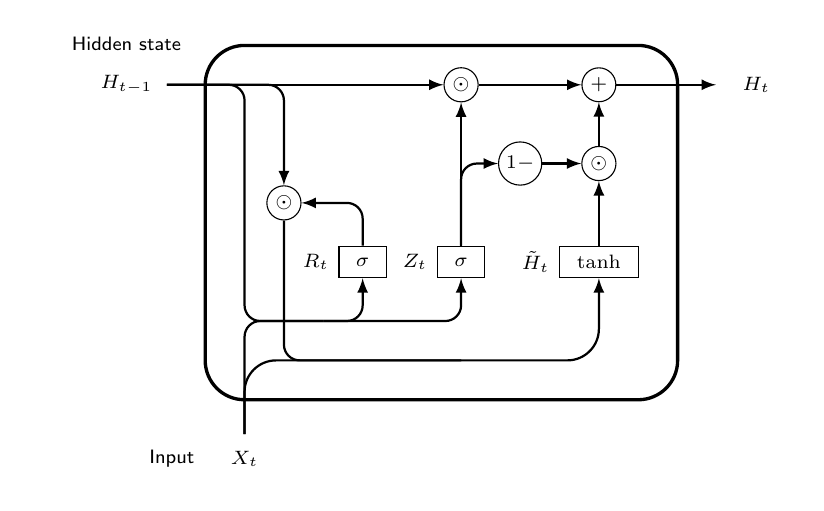
\begin{tikzpicture}[
    font=\sf \scriptsize,
    >=latex,
    % Styles
    cell/.style={
        rectangle,
        rounded corners=5mm,
        draw,
        very thick,
        },
    operator/.style={
        circle,
        draw,
        inner sep=1.5pt,
        minimum height =0.4cm,
        },
    function/.style={
        ellipse,
        draw,
        inner sep=2pt
        },
    ct/.style={
        line width = .75pt,
        minimum height=0.60cm,
        minimum width=1cm,
        inner sep=2pt,
        },
    gt/.style={
        rectangle,
        draw,
        minimum width=0.6cm,
        minimum height=0.4cm,
        inner sep=2pt
        },
    inoutlabels/.style={
        text width=2cm,
        align=center,
        },
    Arrow/.style={
        rounded corners=.2cm,
        thick,
        },
    Arrow2/.style={
        rounded corners=.4cm,
        thick,
        },
    ]

    \node [cell, minimum height =4.5cm, minimum width=6cm] at (0,0){} ;

    \node [gt, label={left:$\boldsymbol{R}_{t}$}] (ibox1) at (-1,-0.5) {$\sigma$};
    \node [gt, label={left:$\boldsymbol{Z}_{t}$}] (ibox2) at (0.25,-0.5) {$\sigma$};
    \node [gt, minimum width=1cm, label={left:$\boldsymbol{\tilde{H}}_{t}$}] (ibox3) at (2,-0.5) {$\tanh$};

    \node [operator] (mux1) at (-2,0.25) {$\odot$};
    \node [operator] (mux2) at (0.25,1.75) {$\odot$};
    \node [operator] (add1) at (2,1.75) {$+$};
    \node [operator] (sub) at (1,0.75) {$1-$};
    \node [operator] (mux3) at (2,0.75) {$\odot$};

    \node[ct, label={[inoutlabels]Hidden state}] (h) at (-4,1.75) {$\boldsymbol{H}_{t-1}$};
    \node[ct, label={[inoutlabels, align=right]left:Input}] (x) at (-2.5,-3) {$\boldsymbol{X}_{t}$};

    \coordinate (inputibox1) at ($ (mux1) + (-0.5,0) $);
    \coordinate (inputibox2) at ($ (ibox1) + (-0.5,-0.75) $);
    \coordinate (midbottom) at ($ (ibox2) + (0,-1.25) $);

    \node[ct] (h2) at (4,1.75) {$\boldsymbol{H}_{t}$};

    %\draw [Arrow] (c) -- (mux1) -- (add1) -- (c2);
    \draw [->, Arrow] (h) -| (mux1);
    \draw [->, Arrow] (h) -- (mux2);
    \draw [->, Arrow] (ibox1) |- (mux1);
    \draw [->, Arrow] (ibox2) -- (mux2);
    \draw [->, Arrow] (ibox2) |- (sub);
    \draw [->, Arrow] (sub) -- (mux3);
    \draw [->, Arrow] (ibox3) -- (mux3);
    \draw [->, Arrow] (mux3) -- (add1);
    \draw [->, Arrow] (mux2) -- (add1);
    \draw [->, Arrow] (add1) -- (h2);

    \draw [-, Arrow] (h) -| (inputibox1) |- (inputibox2);
    \draw [->, Arrow] (inputibox2) -| (ibox1);
    \draw [->, Arrow] (inputibox2) -| (ibox2);
    \draw [-, Arrow] (mux1) |- (midbottom);
    \draw [->, Arrow2] (midbottom) -| (ibox3);
    \draw [-, Arrow2] (x) |- (midbottom);
    \draw [-, Arrow] (x) |- (inputibox2);
\end{tikzpicture}

\end{figure}

As GRUs oferecem uma alternativa competitiva às LSTMs em muitas aplicações, principalmente quando a eficiência no treinamento é um requisito chave, já que ambas têm um desempenho prático semelhante. Além disso, esse modelo possui uma implementação mais simples, dada a menor complexidade de parâmetros a serem operados.

No entanto, as GRUs podem ser mais limitadas em tarefas de NLP que envolvam dependências de longo prazo, já que as LSTMs têm uma estrutura de memória mais robusta capaz de assimilar adequadamente relações distantes em textos. Isso dificulta o uso desse modelo na área de avaliação automática de redações.

\section{Modelos de Linguagem Baseados em Transformadores}

Os modelos de linguagem baseados em transformadores representam uma evolução significativa no campo de NLP. Introduzidos por \citet{attention2017}, foram motivados principalmente pela tarefa de tradução automática de textos, a fim de superar as limitações apresentadas pelas estruturas \textit{encoder-decoder} recorrentes e convolucionais.

A arquitetura dos transformadores é baseada no mecanismo de atenção, que permite ao modelo atribuir diferentes pesos a partes da entrada, codificando a importância de elementos da sequência. Essa abordagem, em especial, possibilita a modelagem de dependências entre a entrada e a saída, flexibilizando a necessidade de recorrência.

Os chamados \textit{transformers} têm se destacado devido a sua eficácia em lidar com tarefas complexas de NLP, como tradução automática, resumo de textos e geração de respostas a perguntas. Além disso, eles são particularmente adequados para lidar com textos extensos, como os de uma redação, ao passo que permitem um processamento paralelo eficiente.

\subsection{Atenção}

A atenção é o cerne dos modelos de transformadores. Esse mecanismo permite assinalar diferentes importâncias aos \textit{tokens} de entrada ao realizar uma tarefa, modelando a dependência entre eles. Seu cálculo considera uma pontuação para cada par de elementos em uma sequência, normalizada pela função \textit{softmax} para obter os pesos.

O mecanismo pode ser representado por meio de uma matriz de atenção, em que cada linha e coluna representam um elemento da sequência. Para o caso dos transformadores, que buscam modelar a relação interna entre os próprios \textit{tokens} de entrada, essa estrutura é chamada matriz de autoatenção. A figura \ref{fig:self_attention} ilustra esse conceito.

\begin{figure}[H]
    \centering
    \caption{Representação de uma matriz de autoatenção com os pesos do primeiro \textit{token} em relação a sua própria frase. Imagem inspirada em \cite{attention2017}.}
    \label{fig:self_attention}
    \begin{minipage}{0.4\textwidth}
        \centering
        

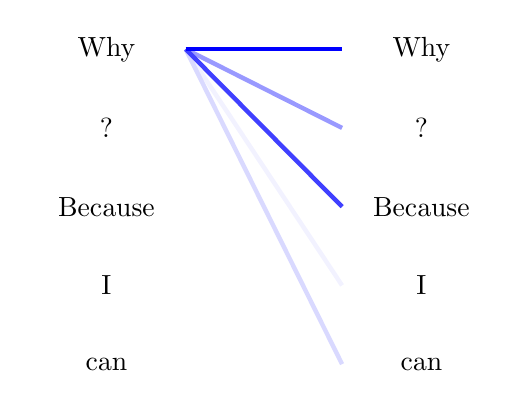
\begin{tikzpicture}[
    y=-1cm,
    every node/.style={minimum width=2cm},
]

    \node (why) at (0,0) {Why};
    \node (int) at (0,1) {?};
    \node (because) at (0,2) {Because};
    \node (i) at (0,3) {I};
    \node (can) at (0,4) {can};

    \node (why2) at (4,0) {Why};
    \node (int2) at (4,1) {?};
    \node (because2) at (4,2) {Because};
    \node (i2) at (4,3) {I};
    \node (can2) at (4,4) {can};

    \draw[-, draw=blue!5, ultra thick] (why.east) -- (i2.west);
    \draw[-, draw=blue!15, ultra thick] (why.east) -- (can2.west);
    \draw[-, draw=blue!40, ultra thick] (why.east) -- (int2.west);
    \draw[-, draw=blue!75, ultra thick] (why.east) -- (because2.west);
    \draw[-, draw=blue!100, ultra thick] (why.east) -- (why2.west);
\end{tikzpicture}

    \end{minipage}
    \begin{minipage}{0.4\textwidth}
        \centering
        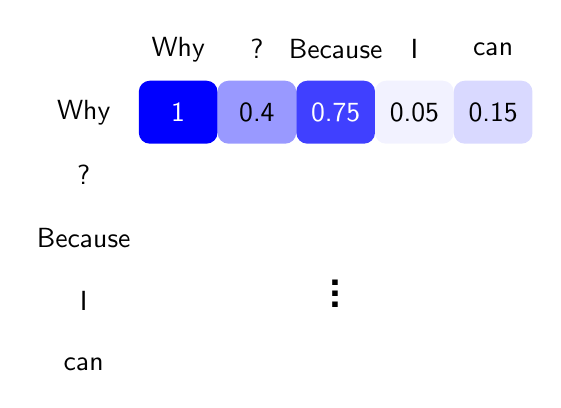
\begin{tikzpicture}[
    y=-1cm,
    every node/.style={font=\sffamily},
    matrixc/.style={fill=blue,rounded corners,minimum height=0.8cm, minimum width=1cm},
]

    \node (why) at (0, 0.8) {Why};
    \node (int) at (0, 1.6) {?};
    \node (because) at (0, 2.4) {Because};
    \node (i) at (0, 3.2) {I};
    \node (can) at (0, 4.0) {can};

    \node (why2) at (1.2, 0) {Why};
    \node (int2) at (2.2, 0) {?};
    \node (because2) at (3.2, 0) {Because};
    \node (i2) at (4.2, 0) {I};
    \node (can2) at (5.2, 0) {can};

    \node[matrixc, text=white] (ww) at (1.2, 0.8) {1};
    \node[matrixc, fill=blue!40] (wint) at (2.2, 0.8) {0.4};
    \node[matrixc, fill=blue!75, text=white] (wb) at (3.2, 0.8) {0.75};
    \node[matrixc, fill=blue!5] (wi) at (4.2, 0.8) {0.05};
    \node[matrixc, fill=blue!15] (wc) at (5.2, 0.8) {0.15};

    % node big dots (...) in matrix middle
    \node (dots) at (3.2, 3) {\Huge $\vdots$};

\end{tikzpicture}

    \end{minipage}
\end{figure}

Matematicamente, dada uma sequência de entrada $\boldsymbol{X} = (x_1, x_2, ..., x_n)$ e uma função de pontuação $a$ que mede a relevância entre dois elementos, a atenção para $x_i$ em relação a um termo $k$ da sequência ($\boldsymbol{A}(x_{i}, x_{k})$) é calculada por \ref{eq:attention}:

\begin{equation}
    \label{eq:attention}
    \boldsymbol{A}(x_{i}, x_{k}) = \frac{e^{a(x_{i}, x_{k})}}{\sum_{j=1}^{n} e^{a(x_{i}, x_{j})}}
\end{equation}

em que $a$ pode ser uma função que compara os elementos, como o produto escalar, por exemplo. Esse processo é executado para todos os elementos da sequência, gerando pesos de atenção que destacam a importância relativa de cada elemento para a tarefa em questão. Os \textit{transformers} utilizam a função \textit{scaled dot-product} para modelar as relações, que será abordada e detalhada mais à frente.

\subsection{Arquitetura}

A arquitetura dos modelos de linguagem baseados em transformadores, conforme proposta por \citet{attention2017}, é caracterizada pela presença de dois módulos principais: o de codificação e o de decodificação. Ambos os componentes são organizados em camadas empilhadas, compreendendo uma estrutura que tem se destacado em tarefas variadas no âmbito do NLP.

No nível de cada camada, a arquitetura incorpora módulos de atenção \textit{multihead}, os quais desempenham um papel fundamental na modelagem de relações de dependência em diferentes partes do contexto. Esses módulos possibilitam a consideração simultânea de informações distantes, promovendo a captura eficiente de padrões sequenciais complexos. Adicionalmente, em cada camada são empregadas redes tradicionais (\textit{feed-forward}) totalmente conectadas, enriquecendo a representação ao permitir a expressão de relações não lineares entre os elementos da sequência.

Além desses elementos, as conexões residuais são introduzidas em cada camada para abordar questões relacionadas à propagação do gradiente. Essas conexões, ao fornecer atalhos na passagem do gradiente, facilitam a otimização em profundidade, promovendo, assim, a eficácia do treinamento em arquiteturas mais extensas.

Após as conexões residuais, são feitas normalizações em cada camada, cujo objetivo é a manutenção da estabilidade e a facilitação da convergência durante o treinamento (\cite{zhang2023dive}). Tal prática contribui para a eficácia do aprendizado ao mitigar possíveis desafios associados à variação na escala dos dados em arquiteturas profundas, como no caso dos \textit{transformers}.

Como os transformadores não possuem uma estrutura sequencial inerente, o modelo incorpora uma etapa de codificação posicional, essencial para fornecer informações sobre a ordem das palavras em uma sequência de entrada. Essa codificação pode ser, ainda, pré-determinada ou aprendida pela rede. Ao adicionar dados de posição às representações vetoriais, a técnica capacita o mecanismo de atenção a antecipar a ordem temporal das palavras, permitindo um melhor desempenho dos \textit{transformers} em contextos linguísticos complexos.

Em suma, os modelos baseados em transformadores apresentam uma configuração estratificada que integra diversos componentes para realizar operações de atenção, conectividade total e normalização, culminando em uma abordagem poderosa para lidar, em especial, com linguagens. A figura \ref{fig:transformer_architecture} ilustra o diagrama de sua arquitetura, em que $N$ é um número arbitrário pré-definido de camadas empilhadas.

\begin{figure}[H]
    \centering
    \caption{Arquitetura de um modelo de linguagem baseado em transformadores. Imagem extraída de \cite{attention2017}.}
    \label{fig:transformer_architecture}
    % Extracted from negrinho/sane_tikz from GitHub (MIT License)
\usetikzlibrary{arrows.meta}
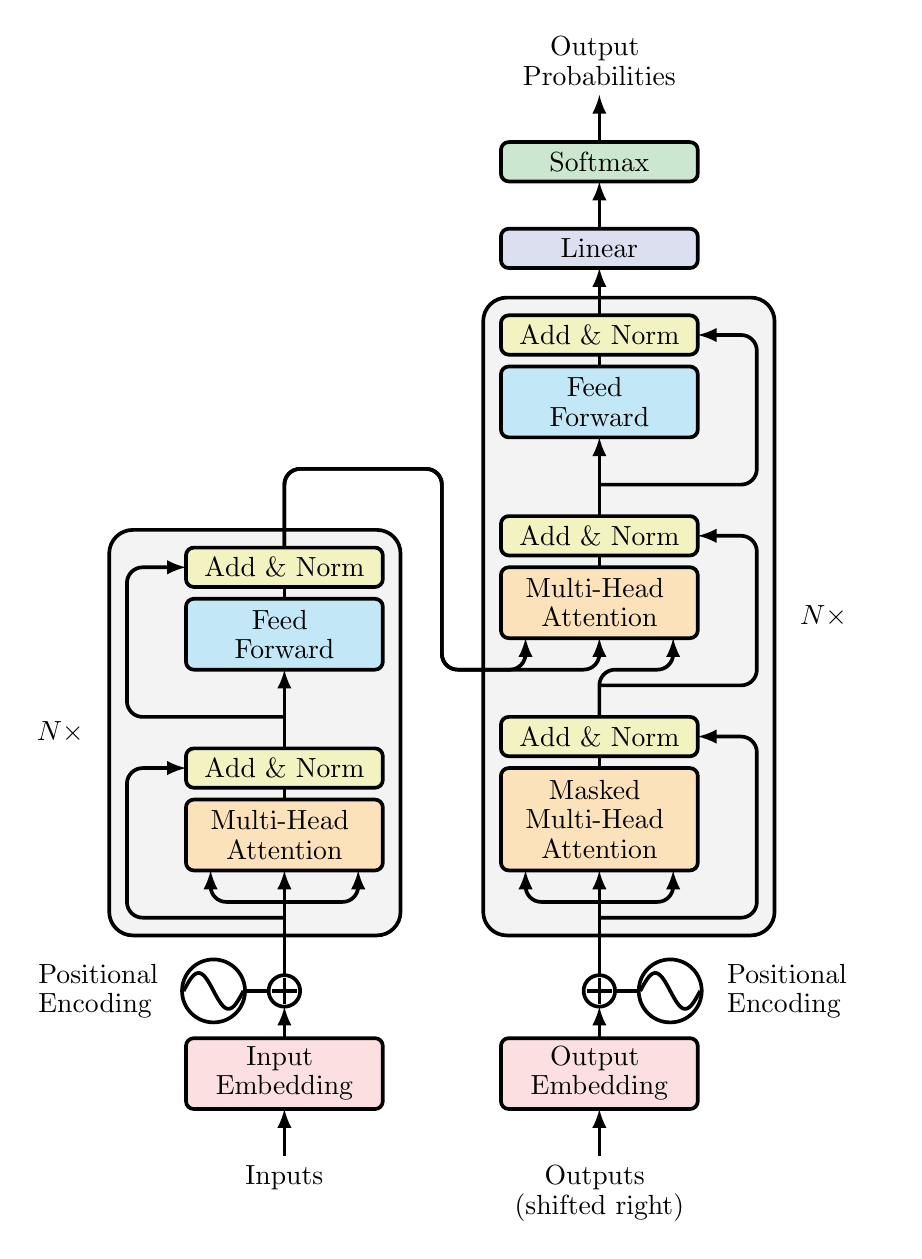
\begin{tikzpicture}
\definecolor{emb_color}{RGB}{252,224,225}
\definecolor{multi_head_attention_color}{RGB}{252,226,187}
\definecolor{add_norm_color}{RGB}{242,243,193}
\definecolor{ff_color}{RGB}{194,232,247}
\definecolor{softmax_color}{RGB}{203,231,207}
\definecolor{linear_color}{RGB}{220,223,240}
\definecolor{gray_bbox_color}{RGB}{243,243,244}
\draw[fill=gray_bbox_color, line width=0.046875cm, rounded corners=0.300000cm] (-0.975000, 6.455000) -- (2.725000, 6.455000) -- (2.725000, 1.305000) -- (-0.975000, 1.305000) -- cycle;
\draw[fill=gray_bbox_color, line width=0.046875cm, rounded corners=0.300000cm] (3.775000, 9.405000) -- (7.475000, 9.405000) -- (7.475000, 1.305000) -- (3.775000, 1.305000) -- cycle;
\draw[line width=0.046875cm, fill=emb_color, rounded corners=0.100000cm] (0.000000, 0.000000) -- (2.500000, 0.000000) -- (2.500000, -0.900000) -- (0.000000, -0.900000) -- cycle;
\node[text width=2.500000cm, align=center] at (1.250000,-0.450000) {Input \vspace{-0.05cm} \linebreak Embedding};
\draw[line width=0.046875cm, fill=emb_color, rounded corners=0.100000cm] (4.000000, 0.000000) -- (6.500000, 0.000000) -- (6.500000, -0.900000) -- (4.000000, -0.900000) -- cycle;
\node[text width=2.500000cm, align=center] at (5.250000,-0.450000) {Output \vspace{-0.05cm} \linebreak Embedding};
\draw[line width=0.046875cm, fill=add_norm_color, rounded corners=0.100000cm] (0.000000, 3.680000) -- (2.500000, 3.680000) -- (2.500000, 3.180000) -- (0.000000, 3.180000) -- cycle;
\node[text width=2.500000cm, align=center] at (1.250000,3.430000) {Add \& Norm};
\draw[line width=0.046875cm, fill=multi_head_attention_color, rounded corners=0.100000cm] (0.000000, 3.030000) -- (2.500000, 3.030000) -- (2.500000, 2.130000) -- (0.000000, 2.130000) -- cycle;
\node[text width=2.500000cm, align=center] at (1.250000,2.580000) {Multi-Head \vspace{-0.05cm} \linebreak Attention};
\draw[line width=0.046875cm] (1.250000, 3.030000) -- (1.250000, 3.180000);
\draw[line width=0.046875cm, fill=add_norm_color, rounded corners=0.100000cm] (4.000000, 6.630000) -- (6.500000, 6.630000) -- (6.500000, 6.130000) -- (4.000000, 6.130000) -- cycle;
\node[text width=2.500000cm, align=center] at (5.250000,6.380000) {Add \& Norm};
\draw[line width=0.046875cm, fill=multi_head_attention_color, rounded corners=0.100000cm] (4.000000, 5.980000) -- (6.500000, 5.980000) -- (6.500000, 5.080000) -- (4.000000, 5.080000) -- cycle;
\node[text width=2.500000cm, align=center] at (5.250000,5.530000) {Multi-Head \vspace{-0.05cm} \linebreak Attention};
\draw[line width=0.046875cm] (5.250000, 5.980000) -- (5.250000, 6.130000);
\draw[line width=0.046875cm, fill=add_norm_color, rounded corners=0.100000cm] (4.000000, 4.080000) -- (6.500000, 4.080000) -- (6.500000, 3.580000) -- (4.000000, 3.580000) -- cycle;
\node[text width=2.500000cm, align=center] at (5.250000,3.830000) {Add \& Norm};
\draw[line width=0.046875cm, fill=multi_head_attention_color, rounded corners=0.100000cm] (4.000000, 3.430000) -- (6.500000, 3.430000) -- (6.500000, 2.130000) -- (4.000000, 2.130000) -- cycle;
\node[text width=2.500000cm, align=center] at (5.250000,2.780000) {Masked \vspace{-0.05cm} \linebreak Multi-Head \vspace{-0.05cm} \linebreak Attention};
\draw[line width=0.046875cm] (5.250000, 3.430000) -- (5.250000, 3.580000);
\draw[line width=0.046875cm, fill=add_norm_color, rounded corners=0.100000cm] (0.000000, 6.230000) -- (2.500000, 6.230000) -- (2.500000, 5.730000) -- (0.000000, 5.730000) -- cycle;
\node[text width=2.500000cm, align=center] at (1.250000,5.980000) {Add \& Norm};
\draw[line width=0.046875cm, fill=ff_color, rounded corners=0.100000cm] (0.000000, 5.580000) -- (2.500000, 5.580000) -- (2.500000, 4.680000) -- (0.000000, 4.680000) -- cycle;
\node[text width=2.500000cm, align=center] at (1.250000,5.130000) {Feed \vspace{-0.05cm} \linebreak Forward};
\draw[line width=0.046875cm] (1.250000, 5.580000) -- (1.250000, 5.730000);
\draw[line width=0.046875cm, fill=add_norm_color, rounded corners=0.100000cm] (4.000000, 9.180000) -- (6.500000, 9.180000) -- (6.500000, 8.680000) -- (4.000000, 8.680000) -- cycle;
\node[text width=2.500000cm, align=center] at (5.250000,8.930000) {Add \& Norm};
\draw[line width=0.046875cm, fill=ff_color, rounded corners=0.100000cm] (4.000000, 8.530000) -- (6.500000, 8.530000) -- (6.500000, 7.630000) -- (4.000000, 7.630000) -- cycle;
\node[text width=2.500000cm, align=center] at (5.250000,8.080000) {Feed \vspace{-0.05cm} \linebreak Forward};
\draw[line width=0.046875cm] (5.250000, 8.530000) -- (5.250000, 8.680000);
\draw[line width=0.046875cm, fill=linear_color, rounded corners=0.100000cm] (4.000000, 10.280000) -- (6.500000, 10.280000) -- (6.500000, 9.780000) -- (4.000000, 9.780000) -- cycle;
\node[text width=2.500000cm, align=center] at (5.250000,10.030000) {Linear};
\draw[line width=0.046875cm, fill=softmax_color, rounded corners=0.100000cm] (4.000000, 11.380000) -- (6.500000, 11.380000) -- (6.500000, 10.880000) -- (4.000000, 10.880000) -- cycle;
\node[text width=2.500000cm, align=center] at (5.250000,11.130000) {Softmax};
\draw[line width=0.046875cm] (1.250000, 0.600000) circle (0.200000);
\draw[line width=0.046875cm] (1.410000, 0.600000) -- (1.090000, 0.600000);
\draw[line width=0.046875cm] (1.250000, 0.760000) -- (1.250000, 0.440000);
\draw[line width=0.046875cm] (5.250000, 0.600000) circle (0.200000);
\draw[line width=0.046875cm] (5.410000, 0.600000) -- (5.090000, 0.600000);
\draw[line width=0.046875cm] (5.250000, 0.760000) -- (5.250000, 0.440000);
\draw[line width=0.046875cm] (0.350000, 0.600000) circle (0.400000);
\draw[line width=0.046875cm] (-0.030000, 0.600000) -- (-0.014490, 0.629156) -- (0.001020, 0.657833) -- (0.016531, 0.685561) -- (0.032041, 0.711884) -- (0.047551, 0.736369) -- (0.063061, 0.758616) -- (0.078571, 0.778258) -- (0.094082, 0.794973) -- (0.109592, 0.808486) -- (0.125102, 0.818576) -- (0.140612, 0.825077) -- (0.156122, 0.827883) -- (0.171633, 0.826946) -- (0.187143, 0.822284) -- (0.202653, 0.813971) -- (0.218163, 0.802145) -- (0.233673, 0.786999) -- (0.249184, 0.768783) -- (0.264694, 0.747796) -- (0.280204, 0.724382) -- (0.295714, 0.698925) -- (0.311224, 0.671845) -- (0.326735, 0.643584) -- (0.342245, 0.614608) -- (0.357755, 0.585392) -- (0.373265, 0.556416) -- (0.388776, 0.528155) -- (0.404286, 0.501075) -- (0.419796, 0.475618) -- (0.435306, 0.452204) -- (0.450816, 0.431217) -- (0.466327, 0.413001) -- (0.481837, 0.397855) -- (0.497347, 0.386029) -- (0.512857, 0.377716) -- (0.528367, 0.373054) -- (0.543878, 0.372117) -- (0.559388, 0.374923) -- (0.574898, 0.381424) -- (0.590408, 0.391514) -- (0.605918, 0.405027) -- (0.621429, 0.421742) -- (0.636939, 0.441384) -- (0.652449, 0.463631) -- (0.667959, 0.488116) -- (0.683469, 0.514439) -- (0.698980, 0.542167) -- (0.714490, 0.570844) -- (0.730000, 0.600000);
\draw[line width=0.046875cm] (6.150000, 0.600000) circle (0.400000);
\draw[line width=0.046875cm] (5.770000, 0.600000) -- (5.785510, 0.629156) -- (5.801020, 0.657833) -- (5.816531, 0.685561) -- (5.832041, 0.711884) -- (5.847551, 0.736369) -- (5.863061, 0.758616) -- (5.878571, 0.778258) -- (5.894082, 0.794973) -- (5.909592, 0.808486) -- (5.925102, 0.818576) -- (5.940612, 0.825077) -- (5.956122, 0.827883) -- (5.971633, 0.826946) -- (5.987143, 0.822284) -- (6.002653, 0.813971) -- (6.018163, 0.802145) -- (6.033673, 0.786999) -- (6.049184, 0.768783) -- (6.064694, 0.747796) -- (6.080204, 0.724382) -- (6.095714, 0.698925) -- (6.111224, 0.671845) -- (6.126735, 0.643584) -- (6.142245, 0.614608) -- (6.157755, 0.585392) -- (6.173265, 0.556416) -- (6.188776, 0.528155) -- (6.204286, 0.501075) -- (6.219796, 0.475618) -- (6.235306, 0.452204) -- (6.250816, 0.431217) -- (6.266327, 0.413001) -- (6.281837, 0.397855) -- (6.297347, 0.386029) -- (6.312857, 0.377716) -- (6.328367, 0.373054) -- (6.343878, 0.372117) -- (6.359388, 0.374923) -- (6.374898, 0.381424) -- (6.390408, 0.391514) -- (6.405918, 0.405027) -- (6.421429, 0.421742) -- (6.436939, 0.441384) -- (6.452449, 0.463631) -- (6.467959, 0.488116) -- (6.483469, 0.514439) -- (6.498980, 0.542167) -- (6.514490, 0.570844) -- (6.530000, 0.600000);
\draw[line width=0.046875cm, -latex] (1.250000, 3.680000) -- (1.250000, 4.680000);
\draw[line width=0.046875cm, -latex] (5.250000, 6.630000) -- (5.250000, 7.630000);
\draw[line width=0.046875cm, -latex] (5.250000, 9.180000) -- (5.250000, 9.780000);
\draw[line width=0.046875cm, -latex] (5.250000, 10.280000) -- (5.250000, 10.880000);
\draw[line width=0.046875cm, -latex] (1.250000, 0.000000) -- (1.250000, 0.400000);
\draw[line width=0.046875cm, -latex] (1.250000, 0.800000) -- (1.250000, 2.130000);
\draw[line width=0.046875cm, -latex] (5.250000, 0.800000) -- (5.250000, 2.130000);
\draw[line width=0.046875cm, -latex] (5.250000, 0.000000) -- (5.250000, 0.400000);
\draw[line width=0.046875cm] (0.750000, 0.600000) -- (1.050000, 0.600000);
\draw[line width=0.046875cm] (5.450000, 0.600000) -- (5.750000, 0.600000);
\draw[-latex, line width=0.046875cm, rounded corners=0.200000cm] (1.250000, 4.080000) -- (-0.750000, 4.080000) -- (-0.750000, 5.980000) -- (0.000000, 5.980000);
\draw[-latex, line width=0.046875cm, rounded corners=0.200000cm] (1.250000, 1.530000) -- (-0.750000, 1.530000) -- (-0.750000, 3.430000) -- (0.000000, 3.430000);
\draw[-latex, line width=0.046875cm, rounded corners=0.200000cm] (5.250000, 1.530000) -- (7.250000, 1.530000) -- (7.250000, 3.830000) -- (6.500000, 3.830000);
\draw[-latex, line width=0.046875cm, rounded corners=0.200000cm] (5.250000, 4.480000) -- (7.250000, 4.480000) -- (7.250000, 6.380000) -- (6.500000, 6.380000);
\draw[-latex, line width=0.046875cm, rounded corners=0.200000cm] (5.250000, 7.030000) -- (7.250000, 7.030000) -- (7.250000, 8.930000) -- (6.500000, 8.930000);
\draw[-latex, line width=0.046875cm, rounded corners=0.200000cm] (1.250000, 1.730000) -- (0.312500, 1.730000) -- (0.312500, 2.130000);
\draw[-latex, line width=0.046875cm, rounded corners=0.200000cm] (1.250000, 1.730000) -- (2.187500, 1.730000) -- (2.187500, 2.130000);
\draw[-latex, line width=0.046875cm, rounded corners=0.200000cm] (5.250000, 1.730000) -- (4.312500, 1.730000) -- (4.312500, 2.130000);
\draw[-latex, line width=0.046875cm, rounded corners=0.200000cm] (5.250000, 1.730000) -- (6.187500, 1.730000) -- (6.187500, 2.130000);
\draw[-latex, line width=0.046875cm, rounded corners=0.200000cm] (1.250000, 6.230000) -- (1.250000, 7.230000) -- (3.250000, 7.230000) -- (3.250000, 4.680000) -- (4.312500, 4.680000) -- (4.312500, 5.080000);
\draw[-latex, line width=0.046875cm, rounded corners=0.200000cm] (1.250000, 6.230000) -- (1.250000, 7.230000) -- (3.250000, 7.230000) -- (3.250000, 4.680000) -- (5.250000, 4.680000) -- (5.250000, 5.080000);
\draw[-latex, line width=0.046875cm, rounded corners=0.200000cm] (5.250000, 4.080000) -- (5.250000, 4.680000) -- (6.187500, 4.680000) -- (6.187500, 5.080000);
\draw[line width=0.046875cm, -latex] (1.250000, -1.500000) -- (1.250000, -0.900000);
\draw[line width=0.046875cm, -latex] (5.250000, -1.500000) -- (5.250000, -0.900000);
\draw[line width=0.046875cm, -latex] (5.250000, 11.380000) -- (5.250000, 11.980000);
\node[text width=2.500000cm, anchor=north, align=center] at (1.250000,-1.500000) {Inputs};
\node[text width=2.500000cm, anchor=north, align=center] at (5.250000,-1.500000) {Outputs \vspace{-0.05cm} \linebreak (shifted right)};
\node[text width=2.500000cm, anchor=south, align=center] at (5.250000,11.980000) {Output \vspace{-0.05cm} \linebreak Probabilities};
\node[anchor=east] at (-1.175000,3.880000) {$N\times$};
\node[anchor=west] at (7.675000,5.355000) {$N\times$};
\node[text width=2.000000cm, anchor=east] at (0.250000,0.600000) {Positional \vspace{-0.05cm} \linebreak Encoding};
\node[text width=2.000000cm, anchor=west] at (6.750000,0.600000) {Positional \vspace{-0.05cm} \linebreak Encoding};
\end{tikzpicture}

\end{figure}

Na estrutura da figura \ref{fig:transformer_architecture}, à esquerda, estão representados os módulos de codificação, que geralmente são utilizados para gerar representações matemáticas da entrada que capturem relações semânticas. Já à direita, estão os módulos de decodificação, mais focados em tarefas de previsão de \textit{tokens} em frases, geração de textos e elaboração de respostas a perguntas.

O foco deste trabalho é a tarefa de avaliação automática de redações, que envolve, principalmente, a etapa de codificação das produções. A seguir, serão detalhados os mecanismos de atenção multicabeça e as subestruturas dos transformadores.

\subsubsection{\textit{Multihead Attention}}

Em geral, o mecanismo de atenção, conforme \citet{zhang2023dive}, pode ser representado por meio de pares de chave-valor $(k, v)$ e de consultadores $q$, em que podemos utilizar $q$ para obter informações de uma base de dados de diferentes $(k, v)$. Seu cálculo, nesse caso, é dado de acordo com a equação \ref{eq:attention_key_value_query}, em que $\mathcal{D}$ é o conjunto de pares chave-valor ($\mathcal{D} = \{(k_{1}, v_{1}), \cdots, (k_{m}, v_{m})\}$).

\begin{equation}
    \label{eq:attention_key_value_query}
    \boldsymbol{A}(\mathcal{D}, q) = \sum_{i=1}^{m} \boldsymbol{\alpha}(q, k_{i}) v_{i}
\end{equation}

A atenção \textit{multihead} é uma extensão desse mecanismo, que permite que o modelo aprenda diferentes tipos de relações entre os elementos da sequência, ao mesmo tempo em que reduz a complexidade computacional ao considerar uma abordagem paralelizável com matrizes de consultadores ($Q$), chaves ($K$) e valores ($V$) (\cite{attention2017}).

Os pesos, nessa técnica, são calculados por meio de uma projeção linear da entrada, seguida da função de atenção \textit{scaled dot-product} abaixo e de uma projeção linear da saída. O cálculo dessa função utiliza uma escala inversamente proporcional à dimensão dos consultadores e chaves $d_{k}$ (\ref{eq:scaled_dot_product}):

\begin{equation}
    \label{eq:scaled_dot_product}
    \boldsymbol{\alpha}(Q, K) = \text{softmax} \left( \frac{QK^{T}}{\sqrt{d_{k}}} \right)
\end{equation}

O valor da atenção resultante é, então, dado pela equação \ref{eq:multihead_attention}.

\begin{equation}
    \label{eq:multihead_attention}
    \boldsymbol{A}(Q, K, V) = \boldsymbol{\alpha}(Q, K)V
\end{equation}

Ao fim, o resultado de cada cabeça é concatenado e novamente projetado linearmente para formar a representação final $\boldsymbol{M}_{a}$, cujo cálculo é dado pela equação \ref{eq:multihead_weights}:

\begin{equation}
    \label{eq:multihead_weights}
    \boldsymbol{M}_{a} = \text{concat}(\boldsymbol{H}_{1}, \cdots, \boldsymbol{H}_{h})W^{O}
\end{equation}

em que $\boldsymbol{H}_{i}$, para $i \in \{1, \cdots, h\}$, é a saída da $i$-ésima cabeça de atenção e $W^{O}$ é uma matriz de pesos. $\boldsymbol{H}_{i}$ é dado, em função de $\boldsymbol{A}$, pela expressão \ref{eq:head_by_attn}.

\begin{equation}
    \label{eq:head_by_attn}
    \boldsymbol{H}_{i} = \boldsymbol{A}(\boldsymbol{Q}_{i}W_{i}^{Q}, \boldsymbol{K}_{i}W_{i}^{K}, \boldsymbol{V}_{i}W_{i}^{V})
\end{equation}

Em que $W_{i}^{Q}$, $W_{i}^{K}$ e $W_{i}^{V}$ são matrizes de pesos e $\boldsymbol{Q}_{i}$, $\boldsymbol{K}_{i}$ e $\boldsymbol{V}_{i}$ são vetores de consultadores, chaves e valores da $i$-ésima cabeça, respectivamente. A figura \ref{fig:multihead_attention} ilustra o cálculo da atenção \textit{multihead}.

\begin{figure}[H]
    \centering
    \caption{À direita, o cálculo da atenção \textit{multihead}. À esquerda, a função de atenção \textit{scaled dot-product}. Imagem adaptada de \cite{attention2017}.}
    \label{fig:multihead_attention}
    \begin{minipage}{0.35\textwidth}
        \centering
        % Adapted from Devin-Taylor/TikZ from GitHub (MIT License)
\usetikzlibrary{calc, backgrounds, arrows.meta}

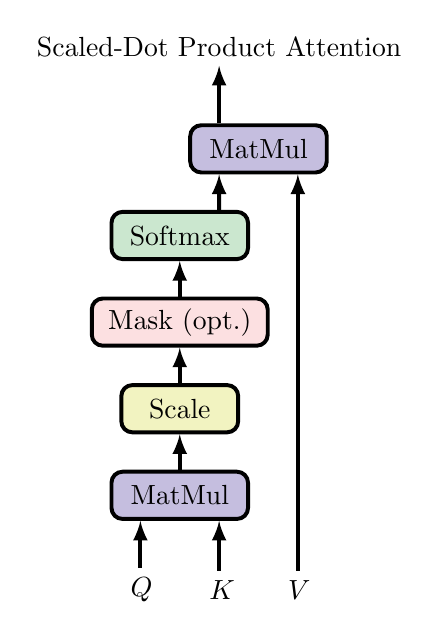
\begin{tikzpicture}[
    >=latex,
]

\definecolor{matmul_color}{RGB}{197,190,223}
\definecolor{emb_color}{RGB}{252,224,225}
\definecolor{add_norm_color}{RGB}{242,243,193}
\definecolor{softmax_color}{RGB}{203,231,207}

\tikzstyle{sqr} = [rectangle, rounded corners, minimum width=1cm, text width=1.25cm, minimum height=.6cm,text centered, draw=black, line width=.5mm]

\node (Q) [text width=.25cm] {$Q$};
\node (K) [text width=.25cm, right of=Q] {$K$};
\node (V) [text width=.25cm, right of=K] {$V$};

\node (matmul) [sqr, fill=matmul_color, above of=K, xshift=-0.5cm, text width=1.5cm, yshift=0.2cm] {MatMul};
\node (scale) [sqr, fill=add_norm_color, above of=matmul, yshift=0.1cm] {Scale};
\node (mask) [sqr, fill=emb_color, above of=scale, yshift=0.1cm, text width=2cm] {Mask (opt.)};
\node (softmax) [sqr, fill=softmax_color, above of=mask, yshift=0.1cm, text width=1.5cm] {Softmax};

\node (matmul2) [sqr, fill=matmul_color, above of=softmax, yshift=0.1cm, xshift=1cm, text width=1.5cm] {MatMul};
\node (scaleddot) [above of=matmul2, yshift=.3cm, xshift=-0.5cm] {Scaled-Dot Product Attention};

\draw[->, line width=.5mm] (matmul.north) -- (scale.south);
\draw[->, line width=.5mm] (scale.north) -- (mask.south);
\draw[->, line width=.5mm] (mask.north) -- (softmax.south);
\draw[->, line width=.5mm] ($ (softmax.north) + (0.5, 0) $) -- ($ (matmul2.south) + (-0.5, 0) $);

\draw[->, line width=.5mm] (Q) -- ($ (matmul.south) + (-0.5, 0) $);
\draw[->, line width=.5mm] (K) -- ($ (matmul.south) + (0.5, 0) $);
\draw[->, line width=.5mm] (V) -- ($ (matmul2.south) + (0.5, 0) $);

\draw[->, line width=.5mm] ($ (matmul2.north) + (-0.5, 0) $) -- (scaleddot.south);

\end{tikzpicture}

    \end{minipage}
    \begin{minipage}{0.5\textwidth}
        \centering
        % Adapted from Devin-Taylor/TikZ from GitHub (MIT License)
\usetikzlibrary{calc, backgrounds, arrows.meta}

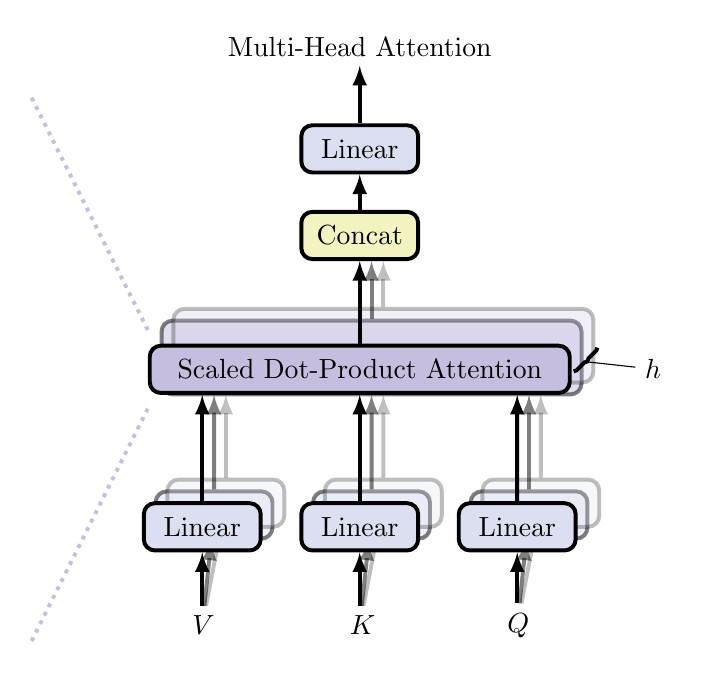
\begin{tikzpicture}[
    >=latex,
]

\definecolor{attention_func_color}{RGB}{197,190,223}
\definecolor{emb_color}{RGB}{252,224,225}
\definecolor{add_norm_color}{RGB}{242,243,193}
\definecolor{linear_color}{RGB}{220,223,240}

\tikzstyle{sqr} = [rectangle, rounded corners, minimum width=1cm, text width=1.25cm, minimum height=.6cm,text centered, draw=black, line width=.5mm]

\node (l1) [sqr, fill=linear_color] {Linear};
\node (V) [text width=.25cm, below of=l1, yshift=-.25cm] {$V$};
\begin{scope}[on  background layer]
\node (l11) [sqr, fill=linear_color, xshift=.15cm, yshift=.15cm, opacity=.5] {};
\draw[->, line width=.5mm, opacity=.5] (V) -- (l11);
\node (l12) [sqr, fill=linear_color, xshift=.3cm, yshift=.3cm, opacity=.25] {};
\draw[->, line width=.5mm, opacity=.25] (V) -- (l12);
\end{scope}

\node (l2) [sqr, fill=linear_color, right of=l1, xshift=1cm] {Linear};
\node (K) [text width=.25cm, below of=l2, yshift=-.25cm] {$K$};
\begin{scope}[on  background layer]
\node (l21) [sqr, fill=linear_color, right of=l1, xshift=1.15cm, yshift=.15cm, opacity=.5] {};
\draw[->, line width=.5mm, opacity=.5] (K) -- (l21);
\node (l22) [sqr, fill=linear_color, right of=l1, xshift=1.3cm, yshift=.3cm, opacity=.25] {};
\draw[->, line width=.5mm, opacity=.25] (K) -- (l22);
\end{scope}

\node (l3) [sqr, fill=linear_color, right of=l2, xshift=1cm] {Linear};
\node (Q) [text width=.25cm, below of=l3, yshift=-.25cm] {$Q$};
\begin{scope}[on  background layer]
\node (l31) [sqr, fill=linear_color, right of=l2, xshift=1.15cm, yshift=.15cm, opacity=.5] {};
\draw[->, line width=.5mm, opacity=.5] (Q) -- (l31);
\node (l32) [sqr, fill=linear_color, right of=l2, xshift=1.3cm, yshift=.3cm, opacity=.25] {};
\draw[->, line width=.5mm, opacity=.25] (Q) -- (l32);
\end{scope}

\node (attn) [sqr, fill=attention_func_color, above of=l2, xshift=0cm, text width=5.1cm, yshift=1cm] {Scaled Dot-Product Attention};
\begin{scope}[on  background layer]
    \node (attn1) [sqr, fill=attention_func_color, above of=l2, xshift=.15cm, text width=5.1cm, text height=2em, yshift=1.15cm, opacity=.5] {};
\node (attn2) [sqr, fill=attention_func_color, above of=l2, xshift=.3cm, text width=5.1cm, text height=2em, yshift=1.3cm, opacity=.25] {};
\end{scope}

\node (add1) [sqr, fill=add_norm_color, above of=attn, yshift=.7cm] {Concat};

\node (l4) [sqr, fill=linear_color, above of=add1, yshift=.1cm] {Linear};

\node (multih) [above of=l4, yshift=.3cm] {Multi-Head Attention};

\draw[->, line width=.5mm] (l1) -- ($(attn.south) + (-2cm, 0)$);
\draw[->, line width=.5mm, opacity=.5] (l11) -- ($(attn.south) + (-1.85cm, 0)$);
\draw[->, line width=.5mm, opacity=.25] (l12) -- ($(attn.south) + (-1.7cm, 0)$);

\draw[->, line width=.5mm] (l2) -- ($(attn.south) + (0, 0)$);
\draw[->, line width=.5mm, opacity=.5] (l21) -- ($(attn.south) + (.15cm, 0)$);
\draw[->, line width=.5mm, opacity=.25] (l22) -- ($(attn.south) + (.3cm, 0)$);

\draw[->, line width=.5mm] (l3) -- ($(attn.south) + (2cm, 0)$);
\draw[->, line width=.5mm, opacity=.5] (l31) -- ($(attn.south) + (2.15cm, 0)$);
\draw[->, line width=.5mm, opacity=.25] (l32) -- ($(attn.south) + (2.3cm, 0)$);

\draw[->, line width=.5mm] (attn.north) -- ($(add1.south) + (0, 0)$);
\draw[->, line width=.5mm, opacity=.5] (attn1.north) -- ($(add1.south) + (.15cm, 0)$);
\draw[->, line width=.5mm, opacity=.25] (attn2.north) -- ($(add1.south) + (.3cm, 0)$);

\draw[->, line width=.5mm] (add1) -- (l4);

\draw[->, line width=.5mm] (V) -- (l1);
\draw[->, line width=.5mm] (K) -- (l2);
\draw[->, line width=.5mm] (Q) -- (l3);

\draw[->, line width=.5mm] (l4.north) -- (multih.south);

\draw [decorate,decoration={brace,amplitude=1pt,mirror,raise=1pt},yshift=0pt, line width=.5mm] (attn.east) -- (attn2.east);
\node (h) [text width=.25cm, right of=attn, yshift=0, xshift=2.75cm] {$h$};
\draw [-] ($(attn.east) + (.15cm, .1cm)$) -- (h);

\draw[-, attention_func_color, line width=.5mm, dotted] ($ (attn.west) + (0, 0.5) $) -- ($(attn.west) + (-1.5, +3.5)$);
\draw[-, attention_func_color, line width=.5mm, dotted] ($ (attn.west) + (0, -0.5) $) -- ($(attn.west) + (-1.5, -3.5)$);

\end{tikzpicture}

    \end{minipage}
\end{figure}

\subsubsection{Codificador}

O codificador processa a entrada sequencial e produz uma representação contextualizada para cada elemento. Cada camada desse módulo contém duas subcamadas subsequentes: a de atenção \textit{multihead} e a de redes neurais totalmente conectadas.

A subcamada de atenção \textit{multihead} permite que o modelo aprenda diferentes tipos de relações entre os elementos da sequência já codificados. Cada cabeça opera em uma projeção linear da entrada, e as saídas são concatenadas e novamente projetadas linearmente para formar a representação final $\boldsymbol{X}$, após a normalização e conexão residual de $\boldsymbol{M}_{a}$, conforme mostrado na seção anterior.

Em seguida, a saída é submetida a uma rede neural totalmente conectada, que consiste em duas camadas lineares com uma função de ativação ReLU (indicada pela equação \ref{eq:relu}) entre elas. Essa subcamada permite que o modelo aprenda representações não lineares dos dados, enriquecendo a representação final.

\begin{equation}
    \label{eq:relu}
    f(x) = \max(0, x)
\end{equation}

A saída de uma camada do codificador, então, é dada pela normalização e conexão residual da equação \ref{eq:encoder_layer}:

\begin{equation}
    \label{eq:encoder_layer}
    \boldsymbol{S} = f(\boldsymbol{W_{1}} \boldsymbol{X} + \boldsymbol{b}_{1})\boldsymbol{W_{2}} + \boldsymbol{b}_{2}
\end{equation}

em que $\boldsymbol{W_{1}}$, $\boldsymbol{W_{2}}$, $\boldsymbol{b}_{1}$ e $\boldsymbol{b}_{2}$ são parâmetros da rede neural totalmente conectada (matrizes de pesos e vetores de vieses, nessa ordem) e $f$ é a função de ativação ReLU (\ref{eq:relu}).

\subsubsection{Decodificador}

O decodificador gera uma sequência de saída contextualizada com base na representação do codificador. Assim como no módulo de codificação, cada camada dessa etapa também possui subcamadas de atenção \textit{multihead} e redes neurais totalmente conectadas. O que difere o módulo decodificador, entretanto, é a inclusão de uma nova camada de atenção com máscara antes da entrada das representações codificadas.

A máscara de atenção é utilizada para evitar que o modelo tenha acesso a informações futuras durante a geração da sequência de saída. Ela faz com que o mecanismo de atenção atue nas codificações dos elementos de modo a suprimir antecipações temporais da sequência pelos \textit{transformers}.

O cálculo final de uma camada do codificador é dado de maneira similar ao da seção anterior, com a inclusão das codificações de entrada e da nova etapa de atenção com máscara.

\section{BERT: \textit{Bidirectional Encoder Representations from Transformers}}

Os modelos baseados em transformadores representaram um marco significativo no avanço da área do NLP, redefinindo as fronteiras da compreensão de linguagem por máquinas. Entre as inovações motivadas pelo surgimento dos \textit{transformers}, destaca-se o BERT (\textit{Bidirectional Encoder Representations from Transformers}), um modelo introduzido por \citet{bert2018} que revolucionou o processamento de sequências textuais pelo computador.

O BERT se diferencia ao capturar, de maneira única, o contexto bidirecional das palavras em uma sequência, superando as limitações dos modelos unidirecionais. Sua arquitetura, baseada em múltiplas camadas de transformadores empilhadas, permite uma codificação contextual robusta dos elementos, capturando relações não só com as palavras anteriores, mas também subsequentes.

O processo de pré-treinamento do BERT permite ao modelo compreender contextos de forma sofisticada, promovendo uma representação rica de palavras ou \textit{tokens} em textos. Além disso, a arquitetura pode ser utilizada como base para o treinamento de sistemas especialistas por meio, geralmente, do aprendizado supervisionado. Neste trabalho, por exemplo, o BERT é refinado para atuar como um classificador de textos, com o objetivo de avaliar redações no modelo do ENEM.

A fim de se adequar à diversidade linguística, foram desenvolvidas algumas variações do modelo a partir de seu pré-treinamento em conjuntos de textos específicos de uma dada linguagem. Dentre as versões, destaca-se o BERTimbau, uma variante do BERT com foco no português brasileiro (\cite{bertimbau2020}). As diferentes alternativas existentes demonstram a capacidade de generalização do modelo, que é capaz de aprender particularidades semânticas e sintáticas de diversas línguas.

O BERT representa não apenas um avanço técnico, mas também uma ferramenta essencial para diversas aplicações em NLP, incluindo a tarefa de AES. A seguir, abordaremos brevemente os aspectos de sua arquitetura, o processo de treinamento e refinamento, a variação do modelo para a língua portuguesa e, por fim, como o BERT pode ser usado para atribuir notas às redações do ENEM de forma automática.

\subsection{Arquitetura}
\label{subsec:bert_architecture}

A arquitetura do BERT é meticulosamente projetada para capturar de forma eficaz as relações contextuais em uma sequência de palavras, incorporando transformadores bidirecionais em múltiplas camadas. Cada camada desempenha um papel crucial na codificação contextual, permitindo que o modelo compreenda as dependências tanto à esquerda quanto à direita de cada unidade. A Figura \ref{fig:bert_architecture} esquematiza a arquitetura geral do BERT.

\begin{figure}[H]
    \centering
    \caption{Arquitetura geral do BERT, considerando a codificação dos \textit{tokens} e as camadas de transformadores. Imagem adaptada de \cite{cui-etal-2022-deep}}.
    \label{fig:bert_architecture}
    \usetikzlibrary{positioning, calc, shapes.misc, shapes.geometric, backgrounds}

\definecolor{red-bert}{RGB}{244,204,204}
\definecolor{blue-bert}{RGB}{201,218,248}
\definecolor{darkblue-bert}{RGB}{80, 129, 188}
\definecolor{yellow-bert}{RGB}{255,242,204}
\definecolor{darkyellow-bert}{RGB}{254,217,102}
\definecolor{green-bert}{RGB}{216,234,210}
\definecolor{gray-bert}{RGB}{243,243,243}

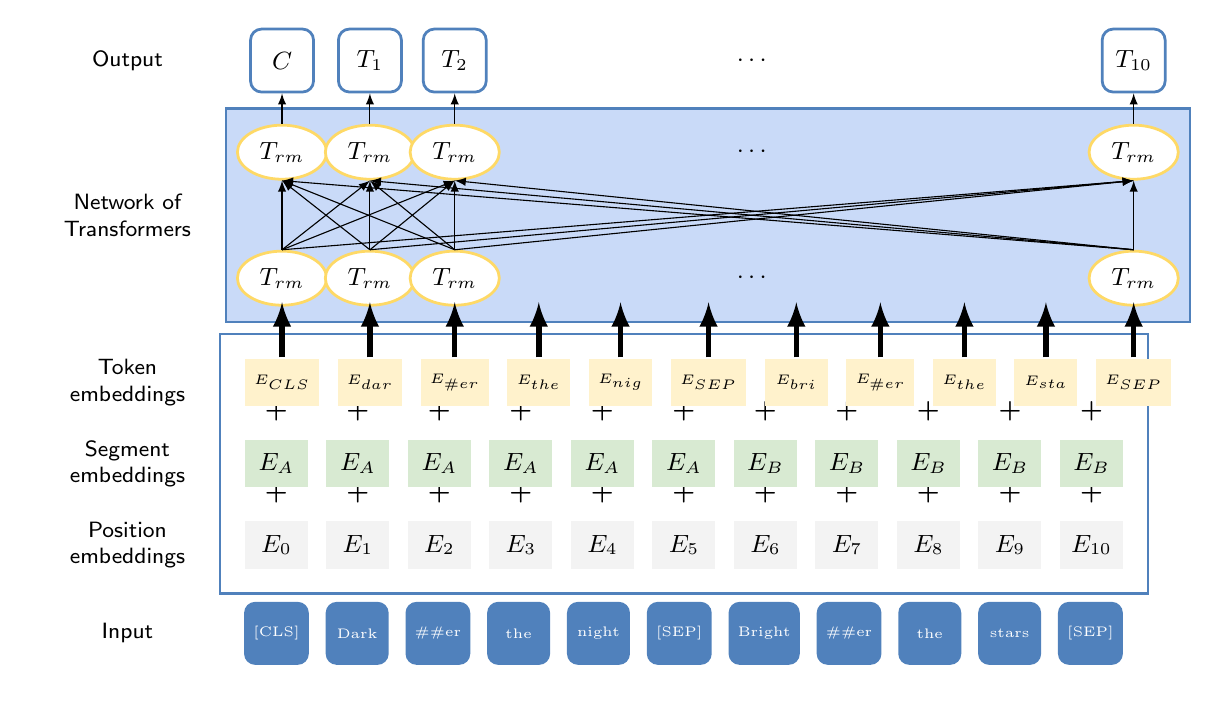
\begin{tikzpicture}[
    node distance=0.2cm,
    >=latex,
    font=\tiny,
    layer-label/.style={text width=2.3cm, minimum height=0.5cm, align=flush center, font=\footnotesize\sffamily},
    token/.style={rectangle, rounded corners, fill=darkblue-bert, text=white, minimum width=8mm, minimum height=8mm},
    posemb/.style={rectangle, fill=gray-bert, minimum height=6mm,minimum width=8mm,line width=1pt, font=\small},
    segemb/.style={rectangle, fill=green-bert, minimum height=6mm,minimum width=8mm,line width=1pt, font=\small},
    toks/.style={rectangle, fill=yellow-bert, minimum height=6mm,minimum width=8mm,line width=1pt, font=\tiny},
    transformer/.style={ellipse, fill=white, draw=darkyellow-bert, minimum height=6mm,minimum width=8mm,line width=1pt, font=\small},
    outnd/.style={rectangle, rounded corners, draw=darkblue-bert, minimum height=8mm,minimum width=8mm,line width=1pt, font=\small},
    ]
]

    \node[layer-label, minimum height=1cm] (input-label) {Input};
    \node[layer-label, above=of input-label] (embedding-label) {Position embeddings};
    \node[layer-label, above=of embedding-label] (encoder-label) {Segment embeddings};
    \node[layer-label, above=of encoder-label] (token-label) {Token embeddings};
    \node[layer-label, above=of token-label, minimum height=3cm] (transformer-label) {Network of Transformers};
    \node[layer-label, above=of transformer-label] (output-label) {Output};

    % The darker the night, the brighter the stars
    \node[token, right=of input-label] (inp-0) {[CLS]};
    \node[token, right=of inp-0] (inp-1) {Dark};
    \node[token, right=of inp-1] (inp-2) {\#\#er};
    \node[token, right=of inp-2] (inp-3) {the};
    \node[token, right=of inp-3] (inp-4) {night};
    \node[token, right=of inp-4] (inp-5) {[SEP]};
    \node[token, right=of inp-5] (inp-6) {Bright};
    \node[token, right=of inp-6] (inp-7) {\#\#er};
    \node[token, right=of inp-7] (inp-8) {the};
    \node[token, right=of inp-8] (inp-9) {stars};
    \node[token, right=of inp-9] (inp-10) {[SEP]};

    % Position embeddings
    \node[posemb, above=of inp-0, right=of embedding-label] (pos-0) {$E_{0}$};
    \node[posemb, right=of pos-0] (pos-1) {$E_{1}$};
    \node[posemb, right=of pos-1] (pos-2) {$E_{2}$};
    \node[posemb, right=of pos-2] (pos-3) {$E_{3}$};
    \node[posemb, right=of pos-3] (pos-4) {$E_{4}$};
    \node[posemb, right=of pos-4] (pos-5) {$E_{5}$};
    \node[posemb, right=of pos-5] (pos-6) {$E_{6}$};
    \node[posemb, right=of pos-6] (pos-7) {$E_{7}$};
    \node[posemb, right=of pos-7] (pos-8) {$E_{8}$};
    \node[posemb, right=of pos-8] (pos-9) {$E_{9}$};
    \node[posemb, right=of pos-9] (pos-10) {$E_{10}$};

    \foreach \i in {0,...,10} {
        \node[above=of pos-\i, yshift=-0.3em] (sum1-\i) {\small \textbf{+}};
    }

    % Segment embeddings
    \node[segemb, above=of pos-0, right=of encoder-label] (seg-0) {$E_{A}$};
    \node[segemb, right=of seg-0] (seg-1) {$E_{A}$};
    \node[segemb, right=of seg-1] (seg-2) {$E_{A}$};
    \node[segemb, right=of seg-2] (seg-3) {$E_{A}$};
    \node[segemb, right=of seg-3] (seg-4) {$E_{A}$};
    \node[segemb, right=of seg-4] (seg-5) {$E_{A}$};
    \node[segemb, right=of seg-5] (seg-6) {$E_{B}$};
    \node[segemb, right=of seg-6] (seg-7) {$E_{B}$};
    \node[segemb, right=of seg-7] (seg-8) {$E_{B}$};
    \node[segemb, right=of seg-8] (seg-9) {$E_{B}$};
    \node[segemb, right=of seg-9] (seg-10) {$E_{B}$};

    \foreach \i in {0,...,10} {
        \node[above=of seg-\i, yshift=-0.3em] (sum1-\i) {\small \textbf{+}};
    }

    % Token embeddings
    \node[toks, above=of seg-0, right=of token-label] (tok-0) {$E_{CLS}$};
    \node[toks, right=of tok-0] (tok-1) {$E_{dar}$};
    \node[toks, right=of tok-1] (tok-2) {$E_{\#er}$};
    \node[toks, right=of tok-2] (tok-3) {$E_{the}$};
    \node[toks, right=of tok-3] (tok-4) {$E_{nig}$};
    \node[toks, right=of tok-4] (tok-5) {$E_{SEP}$};
    \node[toks, right=of tok-5] (tok-6) {$E_{bri}$};
    \node[toks, right=of tok-6] (tok-7) {$E_{\#er}$};
    \node[toks, right=of tok-7] (tok-8) {$E_{the}$};
    \node[toks, right=of tok-8] (tok-9) {$E_{sta}$};
    \node[toks, right=of tok-9] (tok-10) {$E_{SEP}$};

    % rectangle in embeddings
    \begin{scope}[on background layer]
    \draw[darkblue-bert, thick] ($ (tok-0.north west) + (-0.3, 0.3) $) rectangle ($ (pos-10.south east) + (0.3, -0.3) $);
    \end{scope}

    % transformers
    \node[transformer, yshift=-0.8cm] (tm-00) at (transformer-label -| tok-0) {$T_{rm}$};
    \node[transformer, yshift=0.8cm] (tm-01) at (transformer-label -| tok-0) {$T_{rm}$};
    \node[transformer] (tm-10) at (tm-00 -| tok-1) {$T_{rm}$};
    \node[transformer] (tm-11) at (tm-01 -| tok-1) {$T_{rm}$};
    \node[transformer] (tm-20) at (tm-00 -| tok-2) {$T_{rm}$};
    \node[transformer] (tm-21) at (tm-01 -| tok-2) {$T_{rm}$};
    \node[transformer] (tm-n0) at (tm-00 -| tok-10) {$T_{rm}$};
    \node[transformer] (tm-n1) at (tm-01 -| tok-10) {$T_{rm}$};

    % draw cdots
    \node (cdots-1) at ($ .5*(tm-11) + .5*(tm-n1) $) {\small \textbf{$\cdots$}};
    \node (cdots-2) at ($ .5*(tm-10) + .5*(tm-n0) $) {\small \textbf{$\cdots$}};

    % draw rectangle around transformers
    \begin{scope}[on background layer]
    \draw[darkblue-bert, fill=blue-bert, thick] ($ (tm-01.north west) + (-0.3, 0.3) $) rectangle ($ (tm-n0.south east) + (0.3, -0.3) $);

    \end{scope}

    % output
    \node[outnd] (out-0) at (output-label -| tm-01) {$C$};
    \node[outnd] (out-1) at (output-label -| tm-11) {$T_{1}$};
    \node[outnd] (out-2) at (output-label -| tm-21) {$T_{2}$};
    \node[outnd] (out-n) at (output-label -| tm-n1) {$T_{10}$};
    \node (cdots-3) at ($ .5*(out-1) + .5*(out-n) $) {\small \textbf{$\cdots$}};

    % connect token embeddings to first transformers
    \foreach \i in {0,...,10} {
        \draw[->, line width=2pt] (tok-\i) -- ($ (tok-\i.north) + (0, 0.7) $);
    }

    % connect transformers
    \foreach \i in {0,...,2} {
        \foreach \j in {0,...,2} {
            \draw[->] (tm-\i0.north) -- (tm-\j1.south);
        }
    }

    \draw[->] (tm-n0.north) -- (tm-n1.south);
    \draw[->] (tm-00.north) -- (tm-n1.south);
    \draw[->] (tm-10.north) -- (tm-n1.south);
    \draw[->] (tm-20.north) -- (tm-n1.south);
    \draw[->] (tm-n0.north) -- (tm-01.south);
    \draw[->] (tm-n0.north) -- (tm-11.south);
    \draw[->] (tm-n0.north) -- (tm-21.south);

    % connect transformers to output
    \foreach \i in {0,...,2} {
        \draw[->] (tm-\i1.north) -- (out-\i.south);
    }
    \draw[->] (tm-n1.north) -- (out-n.south);
\end{tikzpicture}

\end{figure}

Antes de serem processadas pelas camadas de transformadores, as sequências de palavras de entrada são codificadas em \textit{tokens}. A tokenização divide as palavras em unidades menores, permitindo que o modelo lide de maneira mais flexível com diferentes formas e variações linguísticas. A tokenização em subpalavras também ajuda no desafio de lidar com o vocabulário diversificado e a variabilidade morfológica presente em diferentes idiomas.

Alguns \textit{tokens} especiais também são levados em conta na modelagem. O \textit{token} \texttt{[CLS]}, por exemplo, é adicionado ao início de cada sequência e representa a tarefa de classificação da sentença. Já o \textit{token} \texttt{[SEP]} é adicionado ao final de cada sentença, indicando seu fim. Esses elementos especiais são importantes, em particular, na etapa de treinamento, já que tanto pares de pergunta e resposta quanto textos completos a serem classificados podem ser modelados sem mudar o formato da sequência de entrada (\cite{bert2018}).

O BERT mantém, além disso, vetores que codificam a posição e o segmento de cada \textit{token} na sequência, permitindo que o modelo entenda a ordem de palavras e o mecanismo de separação de sentenças. Essas codificações são essenciais para a compreensão de textos, já que a posição das palavras é relevante para o significado.

As camadas de transformadores, então, recebem como entrada os vetores de \textit{tokens}, posição e segmento, codificando relações contextuais entre as palavras. Cada camada, por meio das conexões bidirecionais entre todos os \textit{transformers} anteriores, gera uma representação dos vocábulos de entrada. Isso possibilita ao BERT capturar interações complexas entre os elementos, fornecendo uma compreensão aprimorada de uma sequência. As saídas de todas as camadas são combinadas para formar uma representação final enriquecida.

Os autores \citet{bert2018} propõem duas arquiteturas do BERT: uma basilar ($\text{\textbf{BERT}}_{\text{\textbf{BASE}}}$) de 12 camadas de transformadores empilhadas, com 12 cabeças de atenção em cada uma, e outra estendida ($\text{\textbf{BERT}}_{\text{\textbf{LARGE}}}$) de 24 camadas de transformadores, com 16 cabeças de atenção em cada uma.

\subsection{Pré-treinamento e \textit{Fine-tuning}}

O pré-treinamento é a etapa em que um modelo de linguagem é capaz de aprender aspectos semânticos e contextuais das sequências, a partir de um grande conjunto de dados. Para cumprir esse objetivo, o BERT é submetido a duas tarefas: a predição de palavras mascaradas e a identificação de relação entre duas sentenças (\cite{zhang2023dive}).

A primeira tarefa, chamada \textit{Masked Language Model} (MLM), consiste em mascarar aleatoriamente 15\% dos \textit{tokens} de entrada e treinar o modelo para prever as palavras mascaradas com base no contexto global.  Essa abordagem promove a compreensão bidirecional de uma sequência, já que as relações de dependência interna de um texto são assimiladas à medida que o BERT otimiza seus parâmetros para cumprir tal função.

Já a segunda tarefa, chamada \textit{Next Sentence Prediction} (NSP), envolve a apresentação de pares de sentenças ao modelo, que deve prever se uma ocorre após a outra no texto original. Essa atribuição aprimora a capacidade do BERT de entender relações semânticas, sendo especialmente útil em contextos de resposta a perguntas ou realização de inferências lógicas.

O pré-treinamento do BERT, em \cite{bert2018}, foi realizado a partir de um conjunto de dados de 3,3 bilhões de palavras, das quais 2,5 bilhões são de artigos do Wikipédia em inglês e 800 milhões são do BookCorpus, um compilado de cerca de 7000 livros autopublicados (\cite{zhu2015aligning}). Além disso, para a tokenização das palavras, foram utilizadas as codificações do algoritmo WordPiece (\cite{wu2016googles}), com um vocabulário de 30000 \textit{tokens}.

Após o pré-treinamento, o BERT pode ser ajustado para tarefas específicas por meio de um processo chamado \textit{fine-tuning}. Durante essa etapa, o modelo pode ser acoplado a outras arquiteturas, que são treinadas em conjuntos de dados rotulados de acordo com a tarefa desejada. Uma mesma versão pré-treinada do BERT pode ser aplicada a diferentes tarefas de NLP, uma vez que o modelo pré-treinado já possui uma compreensão sofisticada da linguagem, o que caracteriza essa abordagem, também, como menos computacionalmente custosa.

A figura \ref{fig:bert_training_tuning} ilustra o processo de pré-treinamento e \textit{fine-tuning} do BERT.

\begin{figure}[H]
    \centering
    \caption{Processo de pré-treinamento do BERT, à esquerda, e uso de modelos pré-treinados no \textit{fine-tuning}, à direita. Imagem extraída de \cite{bert2018}.}
    \label{fig:bert_training_tuning}
    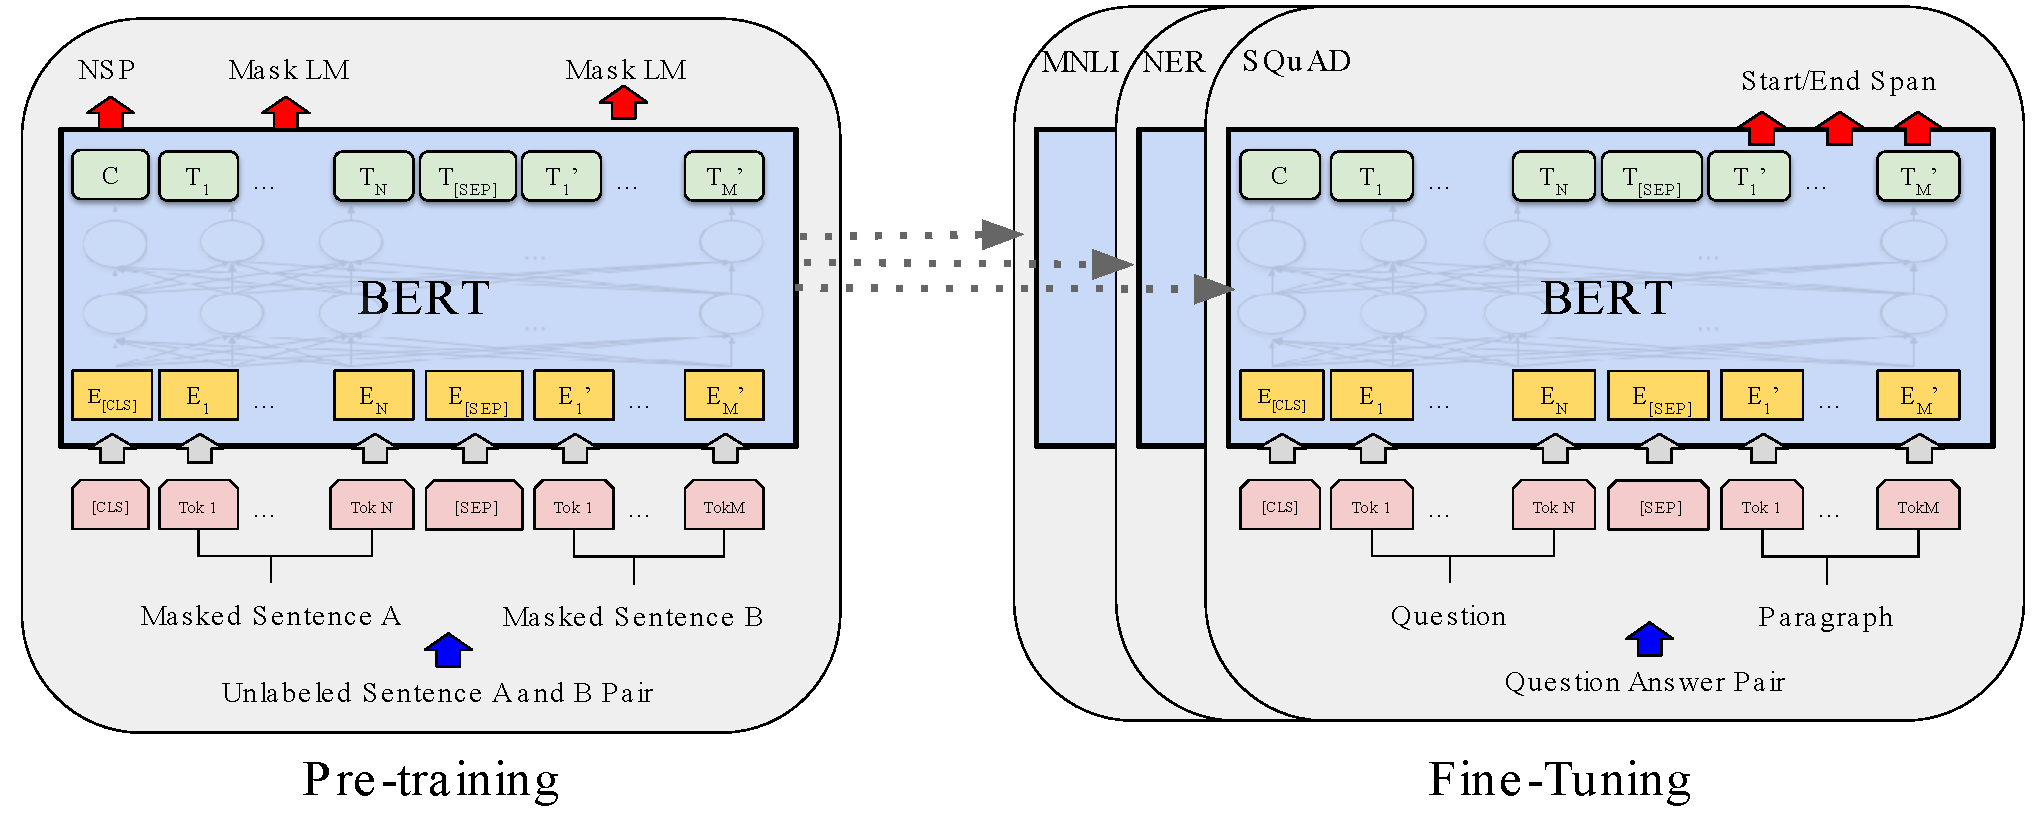
\includegraphics[width=\textwidth]{../figuras/bert_training_tuning}
\end{figure}

\subsection{BERTimbau: BERT para o Português Brasileiro}

A demanda por capturar nuances complexas da língua portuguesa impulsionou o desenvolvimento do BERTimbau, uma adaptação do BERT para o português brasileiro (\cite{bertimbau2020}). Sem alterar a arquitetura ou o processo de pré-treinamento, essa versão usa uma base de textos distinta para ajustar os pesos do modelo, aprendendo a lidar com o vocabulário nacional.

O BERTimbau foi treinado utilizando o conjunto de dados brWaC (\cite{filho-etal-2018-brwac}), uma extensa coleção de textos em português extraídos e filtrados de páginas da web. A base é formada por 2,7 bilhões de \textit{tokens}, que foram reprocessados por \citet{bertimbau2020} para a retirada de \textit{mojibakes}\footnote{Os \textit{mojibakes} são anomalias que acometem textos da internet devido a erros de interpretação de caracteres em diferentes codificações. A exemplo, a palavra "redação", na codificação UTF-8, será mostrada como "redação", na codificação ISO-8859-1. Esses problemas são, em particular, comuns na língua portuguesa devido à riqueza em acentuação.} e \textit{tags} de marcação reminescentes.

A tokenização do conjunto de dados, crucial para lidar com a morfologia variada do português, foi realizada pelo algoritmo SentencePiece (\cite{kudo2018sentencepiece}), com posterior conversão para o formato do WordPiece a fim de manter consistência com os \textit{tokens} do BERT original.

O processo de treinamento do BERTimbau foi realizado com as mesmas duas tarefas de \citet{bert2018}, a partir da predição de palavras ocultas em sentenças e da identificação de relação entre duas frases. Essas etapas contribuem, em especial, para a capacidade do modelo em compreender complexidades semânticas do português, aprimorando sua eficácia ao lidar com textos nessa língua. O BERTimbau também está disponível nas variantes basilar e extensa, ambas com a mesma quantidade de parâmetros das versões do BERT original, o que permite adaptações de acordo com a necessidade da tarefa final a ser realizada.

A disponibilidade de um modelo pré-treinado em língua portuguesa proporciona uma base sólida para uma gama de aplicações em contexto nacional, incluindo a avaliação automática de redações no formato do ENEM, explorada nesta monografia.

\subsection{O BERTimbau na Avaliação Automática de Redações do ENEM}

Devido a sua capacidade de capturar relações complexas em textos da língua portuguesa, o BERTimbau pode ser utilizado na tarefa de AES no âmbito do ENEM. Com o modelo, que é responsável por codificar as redações em \textit{embeddings}, é possível obter representações matemáticas ricas em significado, permitindo a utilização de técnicas de aprendizado de máquina capazes de se especializar em atribuir notas aos textos.

Destaca-se, também, que modelos de linguagem como o BERTimbau, que se beneficiam da paralelização, podem ser utilizados para avaliar redações em larga escala de forma relativamente barata, evitando os gargalos logísticos decorrentes de uma correção exclusivamente humana.

Algumas das técnicas de treinamento de sistemas especializados são os algoritmos supervisionados, que podem ser otimizados para seguir um padrão de um conjunto de dados rotulados. O BERTimbau, por exemplo, pode ser acoplado a uma rede neural, treinada para classificar redações de acordo com notas atribuídas por corretores humanos. Tal é a abordagem deste trabalho, que será melhor explorada no capítulo \ref{chap:work}.
